\documentclass{beamer}

% Theme and style
\usetheme{metropolis} % modern clean theme
\usepackage[ngerman]{babel}
\usepackage{graphicx}
\usepackage{caption}
\usepackage{subcaption}
\usepackage{amsmath}
\usepackage{eurosym}
\usepackage{siunitx}
\usepackage{nicefrac}
\usepackage{tikz}
\usetikzlibrary{positioning, shapes, arrows.meta}

\sisetup{locale=DE, per-mode=symbol}
\DeclareSIUnit{\sieuro}{\mbox{\euro}}

%Hyphenation rules
\usepackage{hyphenat}
\hyphenation{Mathe-matik wieder-gewinnen}

% Metadata
\title{Einführung in die Simulation\\DESMO-J Projekt}
\subtitle{Ausfall von Maschinen}
\author{Schmidt L, Schlager A, Weilert A}
\institute{Paris Lodron Universität Salzburg}
\date{\today}

\begin{document}

% Title slide
    \maketitle

% Overview
    \begin{frame}{Overview}
        \tableofcontents
    \end{frame}

% Section: Introduction


    \section{Einführung}
    \begin{frame}{Szenario}
        Eine Fabrik hat $m$ Maschinen und $s$ Service-MitarbeiterInnen.
        Die Maschinen brauchen immer wieder einen Service.
        In dieser Zeit verursachen die Maschinen Kosten, bis ein(e) MitarbeiterIn sie repariert hat.
        Sind alle MitarbeiterInnen beschäftigt,
        müssen die Maschinen auf eine Reparatur warten.
        Die Reparaturreihenfolge erfolgt nach dem FIFO Prinzip.\vspace*{1em}\newline
        \textit{Kosten}
        \begin{itemize}
            \item $\SI{10}{\sieuro\per\hour}$ pro MitarbeiterIn (immer)
            \item $\SI{50}{\sieuro\per\hour}$ pro Maschine (solange außer Betrieb)
        \end{itemize}
    \end{frame}

    \begin{frame}{Kosten}
        Die verursachten Kosten sind von der gesamten Dauer der inaktiven Phasen (\textbf{Downtime} DT) aller Maschinen und den
        Löhnen der MitarbeiterInnen abhängig.
        Sei die Anzahl der Maschinen fix, so ergibt sich die Kostenfunktion in Abhängigkeit von der Anzahl der MitarbeiterInnen,
        der Downtime und der gesamten Dauer der Simulation (\textbf{Total Time} TT).
        \[
            \mathrm{Cost}(s, \text{DT}, \text{TT}) = \text{DT}\,\cdot \SI{50}{\sieuro\per\hour} + \text{TT}\,\cdot \SI{10}{\sieuro\per\hour} \cdot s
        \]
    \end{frame}

    \begin{frame}{Ziel}
        Wir suchen die Anzahl $\hat{s}$ an MitarbeiterInnen, welche die Gesamtkosten für $m$ Maschinen minimiert.
        \[
            \hat{s} = \arg\min_{s \in \mathbb{N}} \mathrm{Cost}(s, \text{DT}, \text{TT})
        \]
        Aus den Ergebnissen für unterschiedliche $m$ soll außerdem ein Richtwert bestimmt werden, welcher
        die optimale Anzahl an MitarbeiterInnen pro Maschine beschreiben soll.
    \end{frame}

% Section: System Description


    \section{System Beschreibung}
    \begin{frame}{Simulation}
        Allgemeine Informationen zur Simulation
        \begin{itemize}
            \item Prozessorientierte Simulation mit Maschinen als Prozesse
            \item Simulationsdauer von 2 Arbeitsjahren (500 Tage, $\SI{8}{\hour}$)
            \item Zeitauflösung in Minuten
            \item $m\in\{1, \dots, 20\}$ und $s\in\{1,\dots, 20\}$
        \end{itemize}
    \end{frame}

    \begin{frame}{Wahrscheinlichkeitverteilungen}
        \begin{itemize}
            \item Zeit bis zum nächsten Breakdown (Uptime): $\mathrm{Exp}(\nicefrac{1}{420})$\\
            8h im Mittel
            \item Reparaturzeit: $\mathrm{Exp}(\nicefrac{1}{120})$\\
            2h im Mittel
        \end{itemize}
    \end{frame}

    \begin{frame}{Fabrikmodell}
        \begin{columns}
            \column{0.48\textwidth}
            \begin{itemize}
                \item zentrales Model der Simulation
                \item verwaltet MitarbeiterInnen
                \item instanziiert \& aktiviert Maschinenprozesse
            \end{itemize}
            \column{0.48\textwidth}
            \begin{figure}
                \centering
                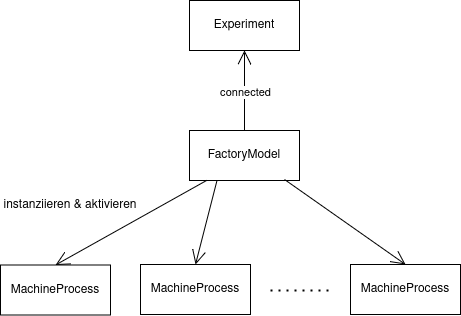
\includegraphics[width=\textwidth]{figures/factory_model_overview}
            \end{figure}
        \end{columns}
    \end{frame}

    \begin{frame}{Maschinenprozess}
        \begin{columns}
            \column{0.48\textwidth}
            \begin{itemize}
                \item \texttt{hold} zur Simulation von normalem Arbeiten \& Reparatur
                \item warten in Repair Queue, falls kein(e) MitarbeiterIn vorhanden ist
                \item auf Reparatur warten durch \texttt{passivate}
            \end{itemize}
            \column{0.48\textwidth}
            \begin{figure}
                \centering
                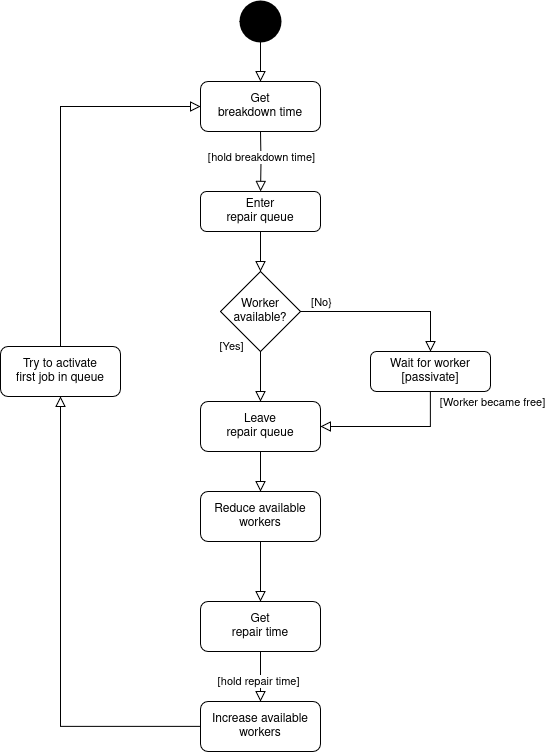
\includegraphics[width=\textwidth]{figures/machine_process}
            \end{figure}
        \end{columns}
    \end{frame}

    \begin{frame}[fragile]{MitarbeiterInnen Modell}
        Einfache Simulation als Zahl
        \begin{itemize}
            \item Sind MitarbeiterInnen verfügbar: \verb|availableWorkers > 0|
            \item Fordere MitarbeiterIn an: \verb|availableWorkers--|
            \item Gib MitarbeiterIn frei: \verb|availableWorkers++|
        \end{itemize}
    \end{frame}

% Section: Implementation


    \section{Implementation in Java}
    \begin{frame}{FactoryModel UML}
        \begin{columns}
            \column{0.48\textwidth}
            \begin{itemize}
                \item Erweitert \texttt{Model} Klasse von DESMO-J
                \item Zugriff auf die Wahrscheinlichkeitsverteilungen
                \item Verwaltung der Reparaturwarteschlange
                \item Methoden zur Verwaltung von MitarbeiterInnen
            \end{itemize}
            \column{0.48\textwidth}
            \begin{figure}
                \centering
                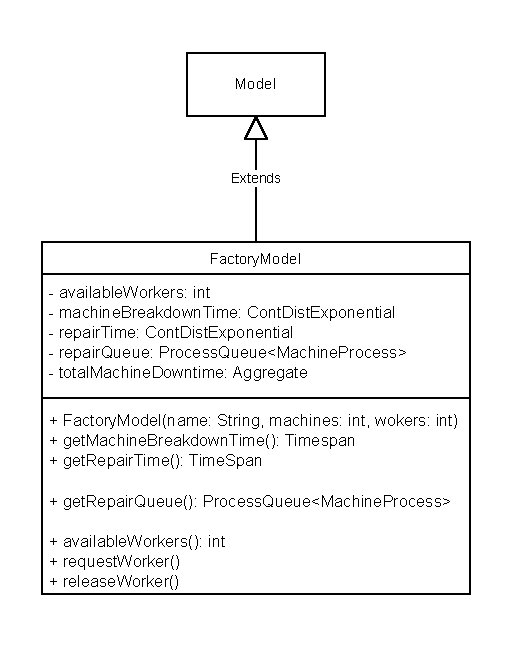
\includegraphics[width=\textwidth]{figures/factorymodel_uml}
            \end{figure}
        \end{columns}
    \end{frame}

    \begin{frame}{FactoryModel}
        \texttt{init}-Methode von \texttt{Model}
        \begin{figure}
            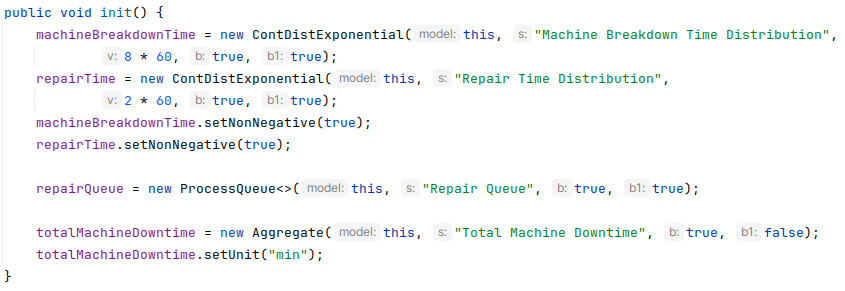
\includegraphics[width=\textwidth]{figures/code/factory_model_init}
        \end{figure}
    \end{frame}
    
    \begin{frame}{FactoryModel}
        \texttt{initialSchedules}-Methode von \texttt{Model}
        \begin{figure}
            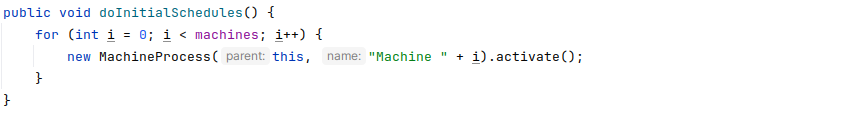
\includegraphics[width=\textwidth]{figures/code/factory_model_initialSchedule}
        \end{figure}
    \end{frame}

    \begin{frame}{FactoryModel}
        Sampling der Wahrscheinlichkeitsverteilungen
        \begin{figure}
            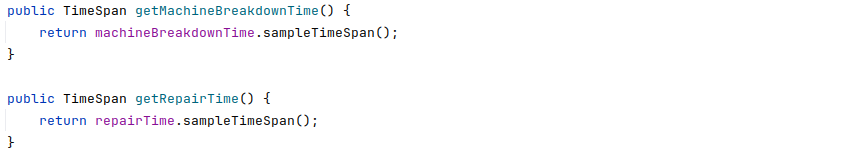
\includegraphics[width=\textwidth]{figures/code/factory_model_time_sample}
        \end{figure}
    \end{frame}

    \begin{frame}{FactoryModel}
        Verwaltung von MitarbeiterInnen
        \begin{figure}
            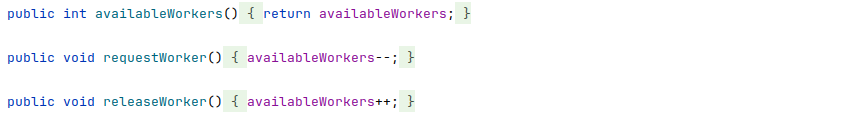
\includegraphics[width=\textwidth]{figures/code/factory_model_worker_methods}
        \end{figure}
    \end{frame}

    \begin{frame}{MachineProcess UML}
        \begin{columns}
            \column{0.48\textwidth}
            \begin{itemize}
                \item Erweitert \texttt{SimProcess} Klasse von DESMO-J
                \item besitzt einen \texttt{lifeCycle}
                \item startet Reparaturen
                \item meldet dem Modell die eigene Downtime
            \end{itemize}
            \column{0.48\textwidth}
            \begin{figure}
                \centering
                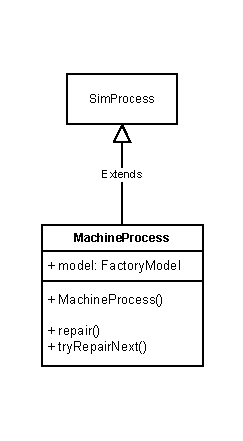
\includegraphics[width=\textwidth]{figures/machine_process_uml}
            \end{figure}
        \end{columns}
    \end{frame}

    \begin{frame}{MachineProcess}
        \texttt{lifeCycle}-Methode von \texttt{SimProcess}
        \begin{figure}
            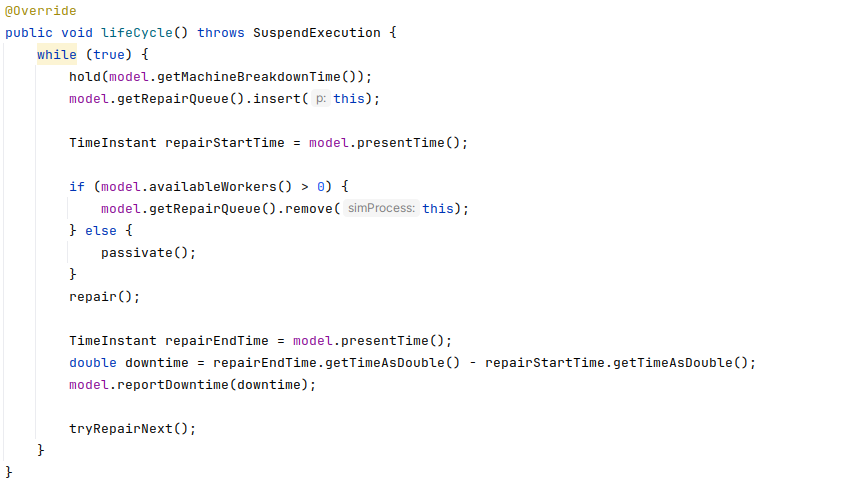
\includegraphics[width=\textwidth]{figures/code/machine_process_lifeCycle}
        \end{figure}
    \end{frame}

    \begin{frame}{MachineProcess}
        Reparatur einer Maschine
        \begin{figure}
            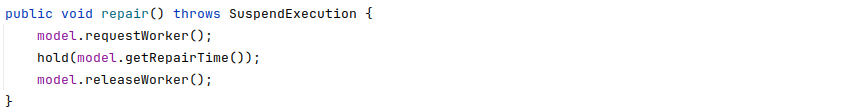
\includegraphics[width=\textwidth]{figures/code/machine_process_repair}
        \end{figure}
    \end{frame}

    \begin{frame}{MachineProcess}
        Aktivierung von wartenden Maschinen
        \begin{figure}
            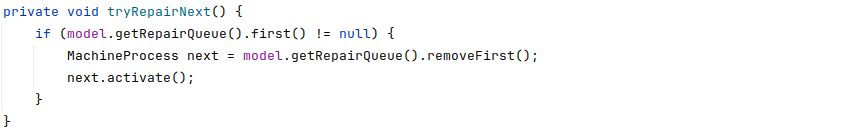
\includegraphics[width=\textwidth]{figures/code/machine_process_tryRepairNext}
        \end{figure}
    \end{frame}

    \begin{frame}{Applikation}
        Ausführung einer einzelnen Simulation
        \begin{figure}
            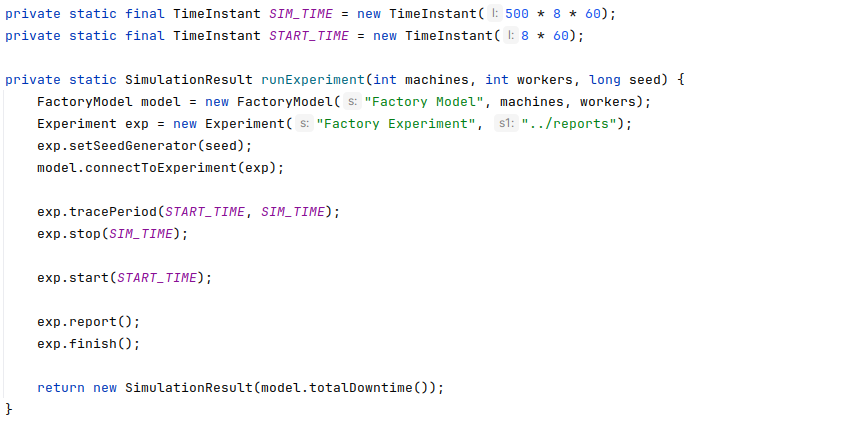
\includegraphics[width=\textwidth]{figures/code/app_run_experiment}
        \end{figure}
    \end{frame}

    \begin{frame}{Applikation}
        Simulation aller Konfigurationen
        \begin{figure}
            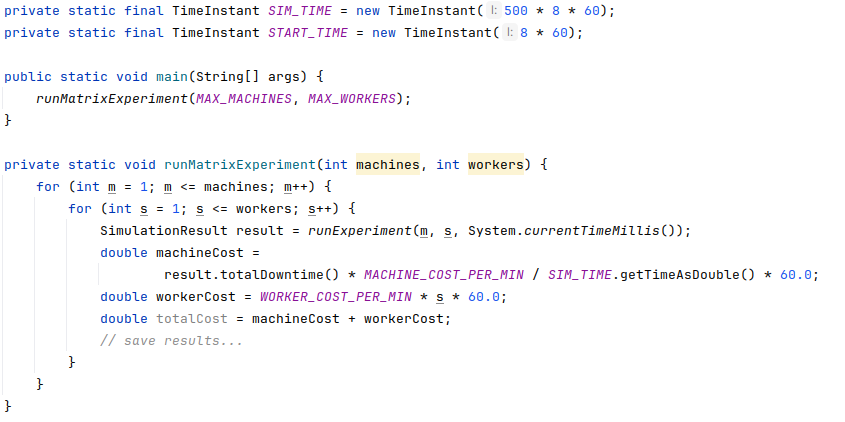
\includegraphics[width=\textwidth]{figures/code/app_main}
        \end{figure}
    \end{frame}

% Section: Results
    \section{Ergebnisse}
    \begin{frame}{Ergebnisse}
        Wir vergleichen die erzeugten \textbf{Kosten der Maschinen und der MitarbeiterInnen} mit den entstehenden
        \textbf{Gesamtkosten}.
    \end{frame}

    %\usepackage{graphicx}
\begin{frame}{Ergebnisse}
    \only<1>{
        \begin{figure}
            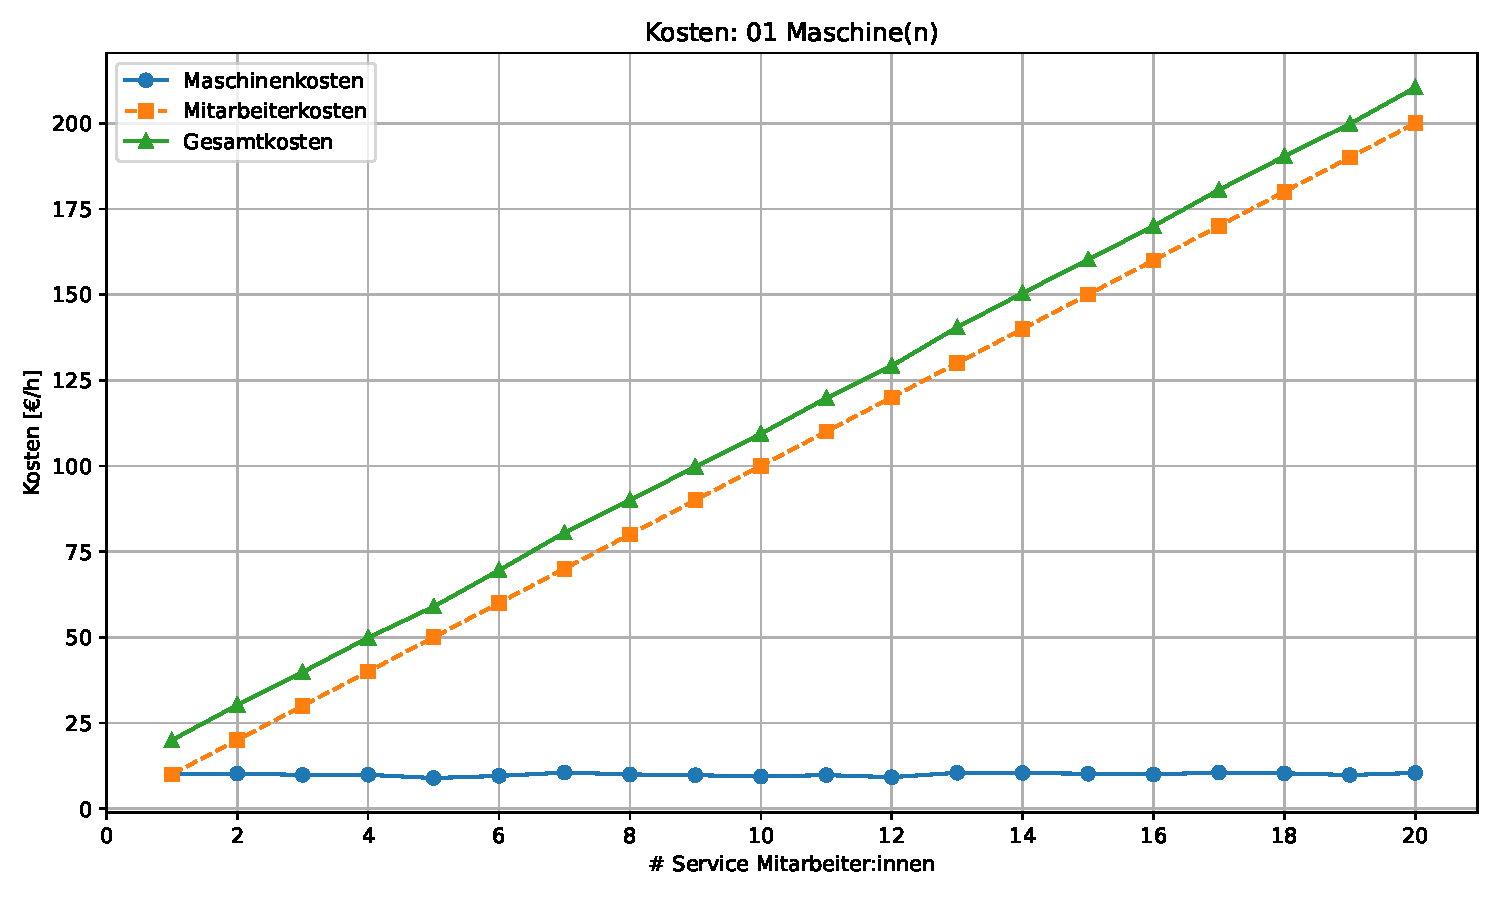
\includegraphics[width=\textwidth]{figures/results/m01_plot}
        \end{figure}
    }
    \only<2>{
        \begin{figure}
            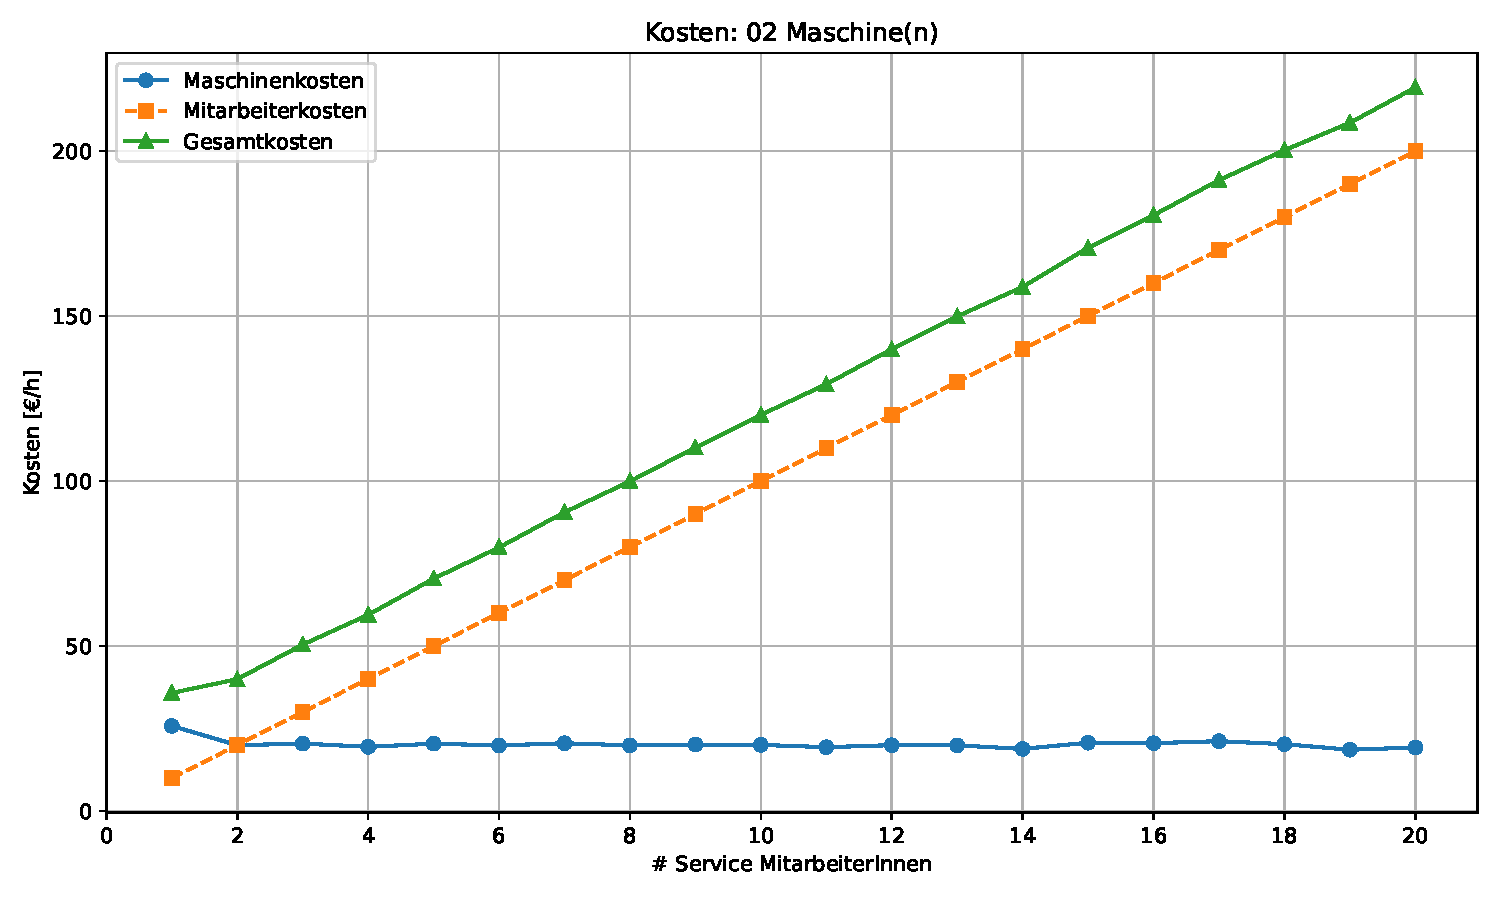
\includegraphics[width=\textwidth]{figures/results/m02_plot}
        \end{figure}
    }
    \only<3>{
        \begin{figure}
            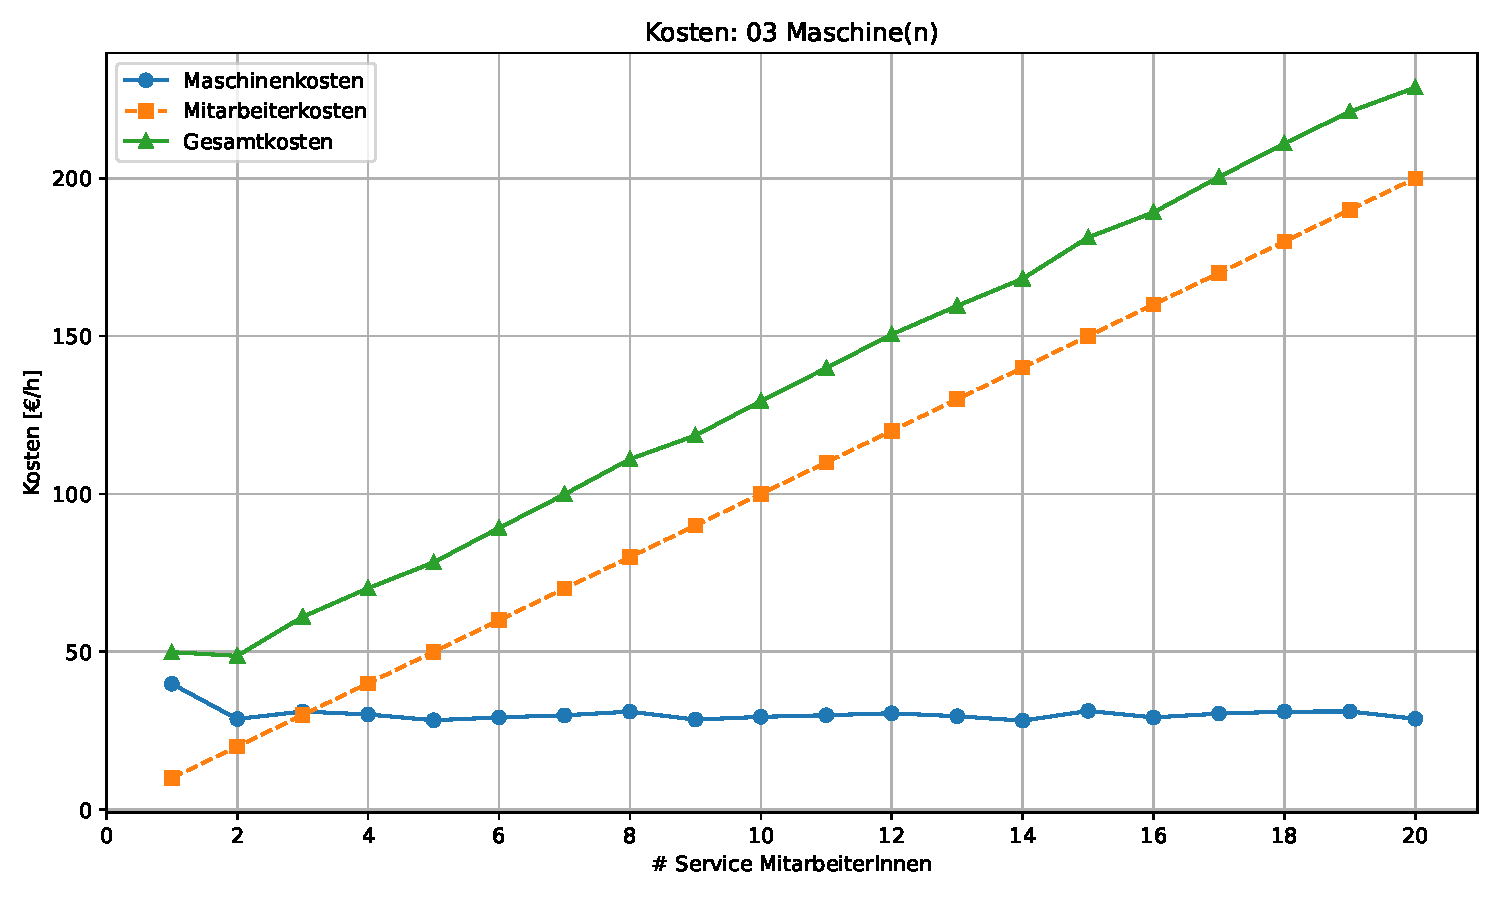
\includegraphics[width=\textwidth]{figures/results/m03_plot}
        \end{figure}
    }
    \only<4>{
        \begin{figure}
            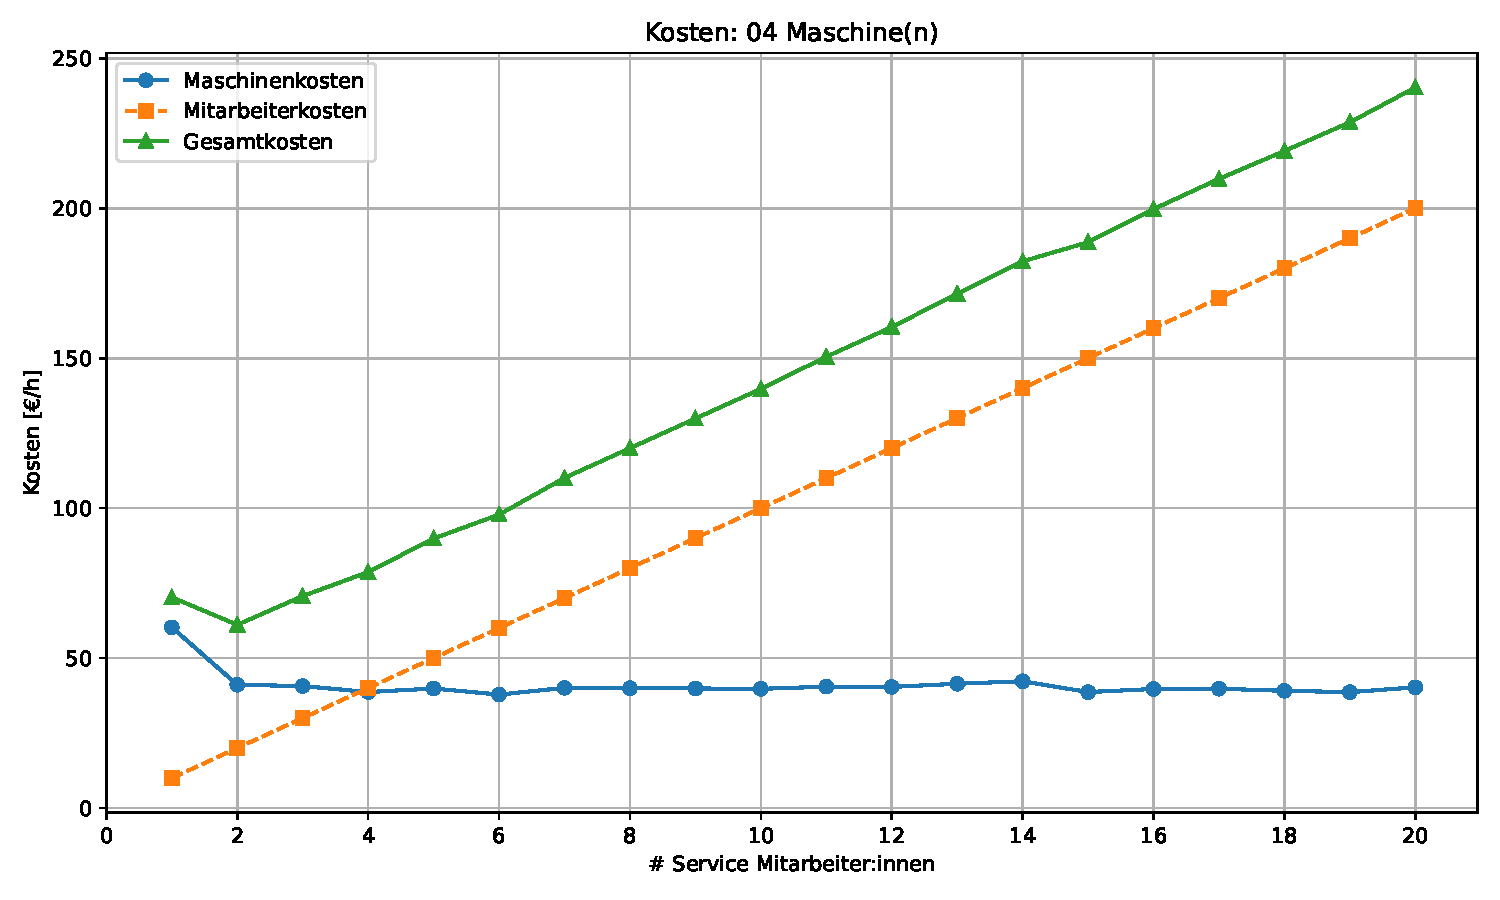
\includegraphics[width=\textwidth]{figures/results/m04_plot}
        \end{figure}
    }
    \only<5>{
        \begin{figure}
            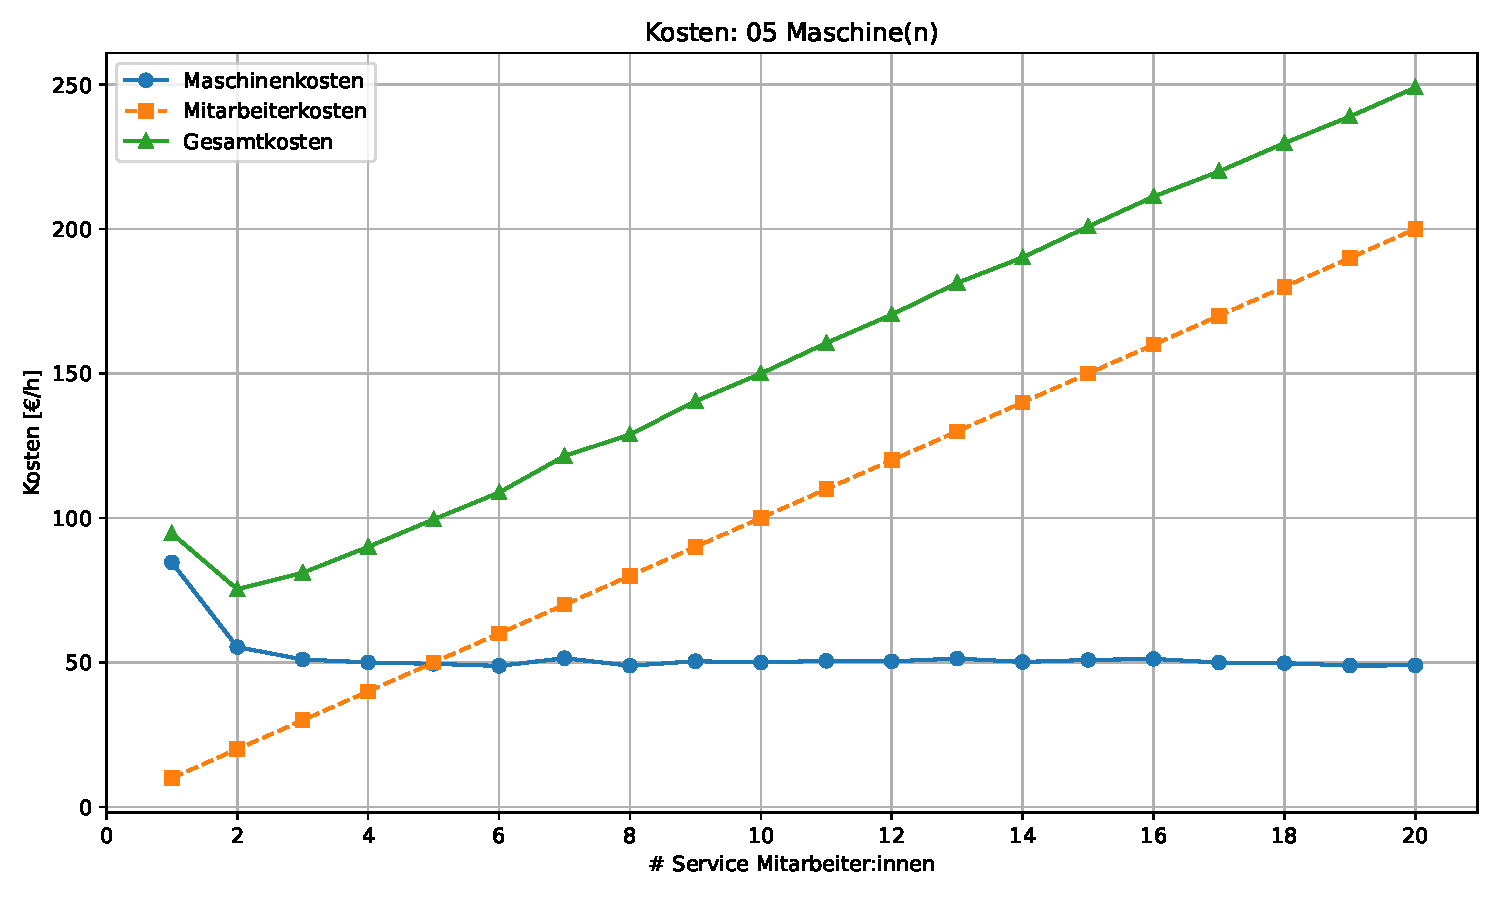
\includegraphics[width=\textwidth]{figures/results/m05_plot}
        \end{figure}
    }
    \only<6>{
        \begin{figure}
            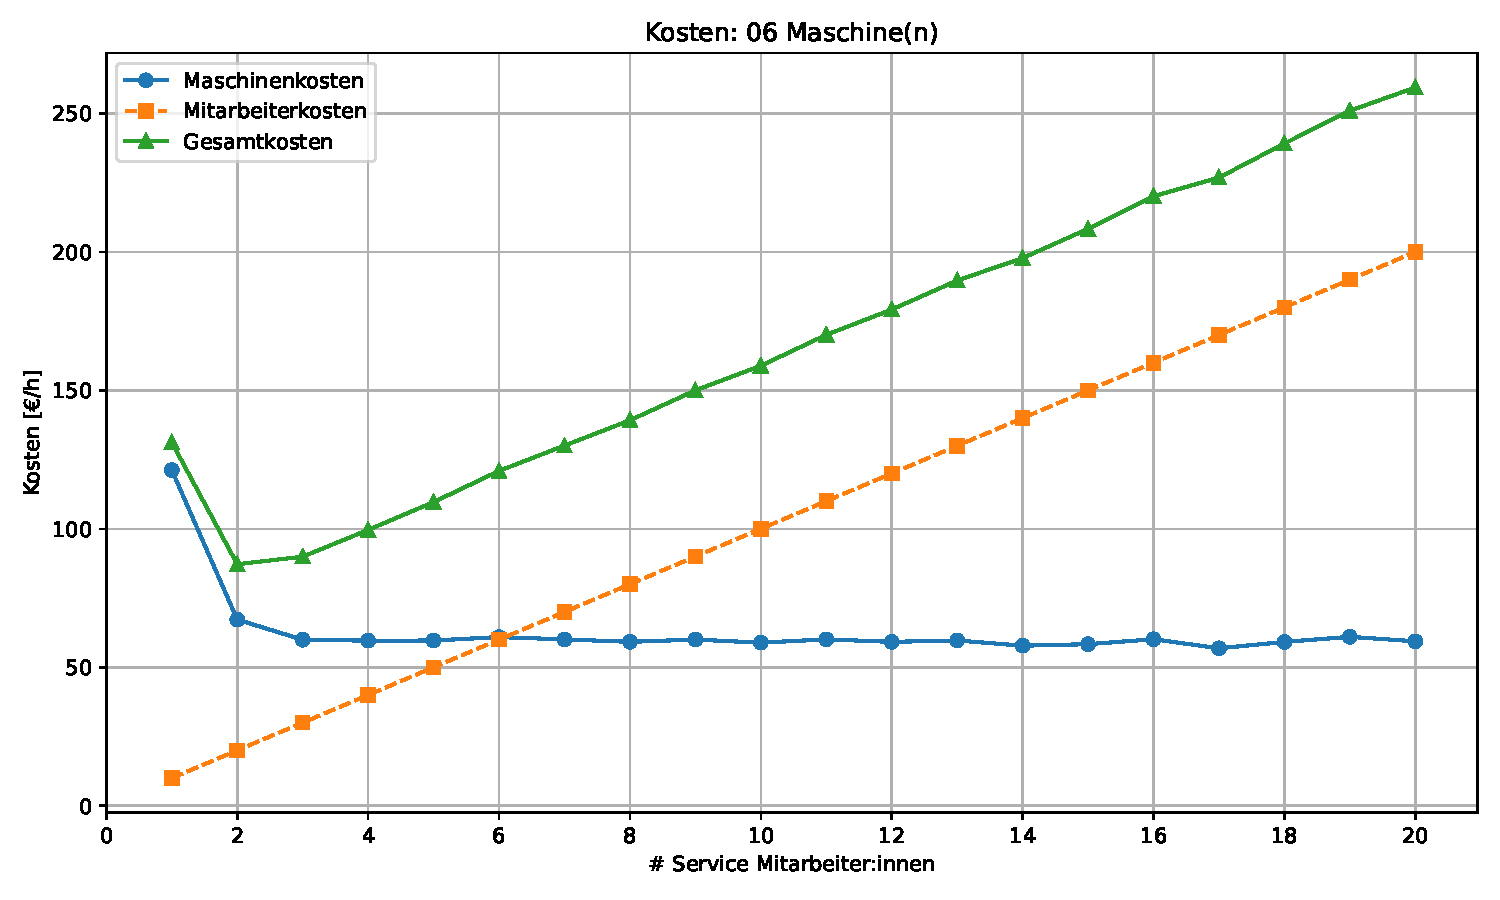
\includegraphics[width=\textwidth]{figures/results/m06_plot}
        \end{figure}
    }
    \only<7>{
        \begin{figure}
            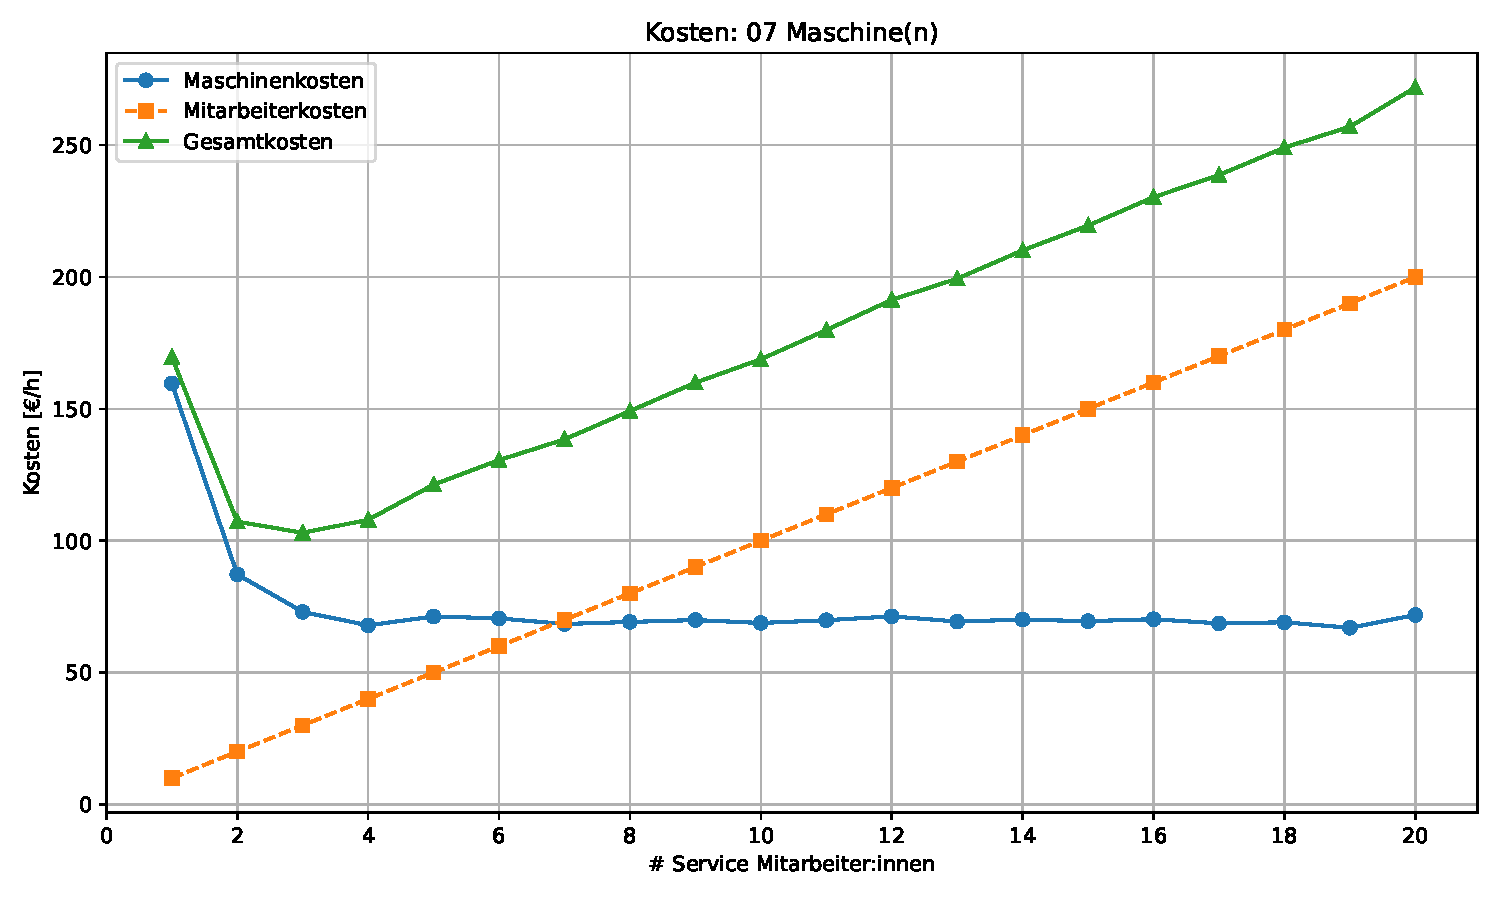
\includegraphics[width=\textwidth]{figures/results/m07_plot}
        \end{figure}
    }
    \only<8>{
        \begin{figure}
            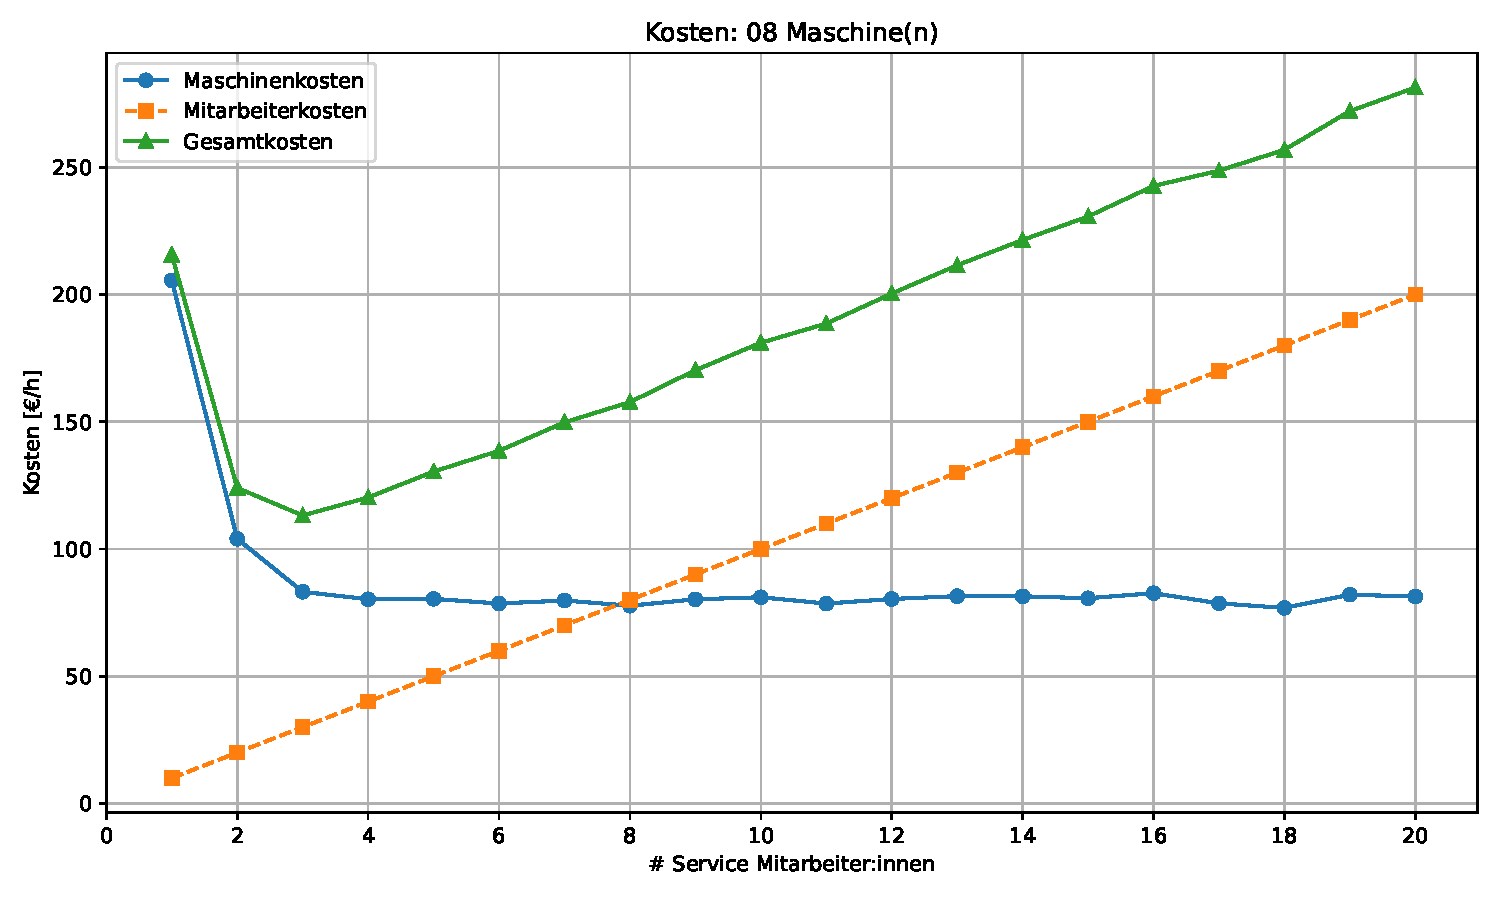
\includegraphics[width=\textwidth]{figures/results/m08_plot}
        \end{figure}
    }
    \only<9>{
        \begin{figure}
            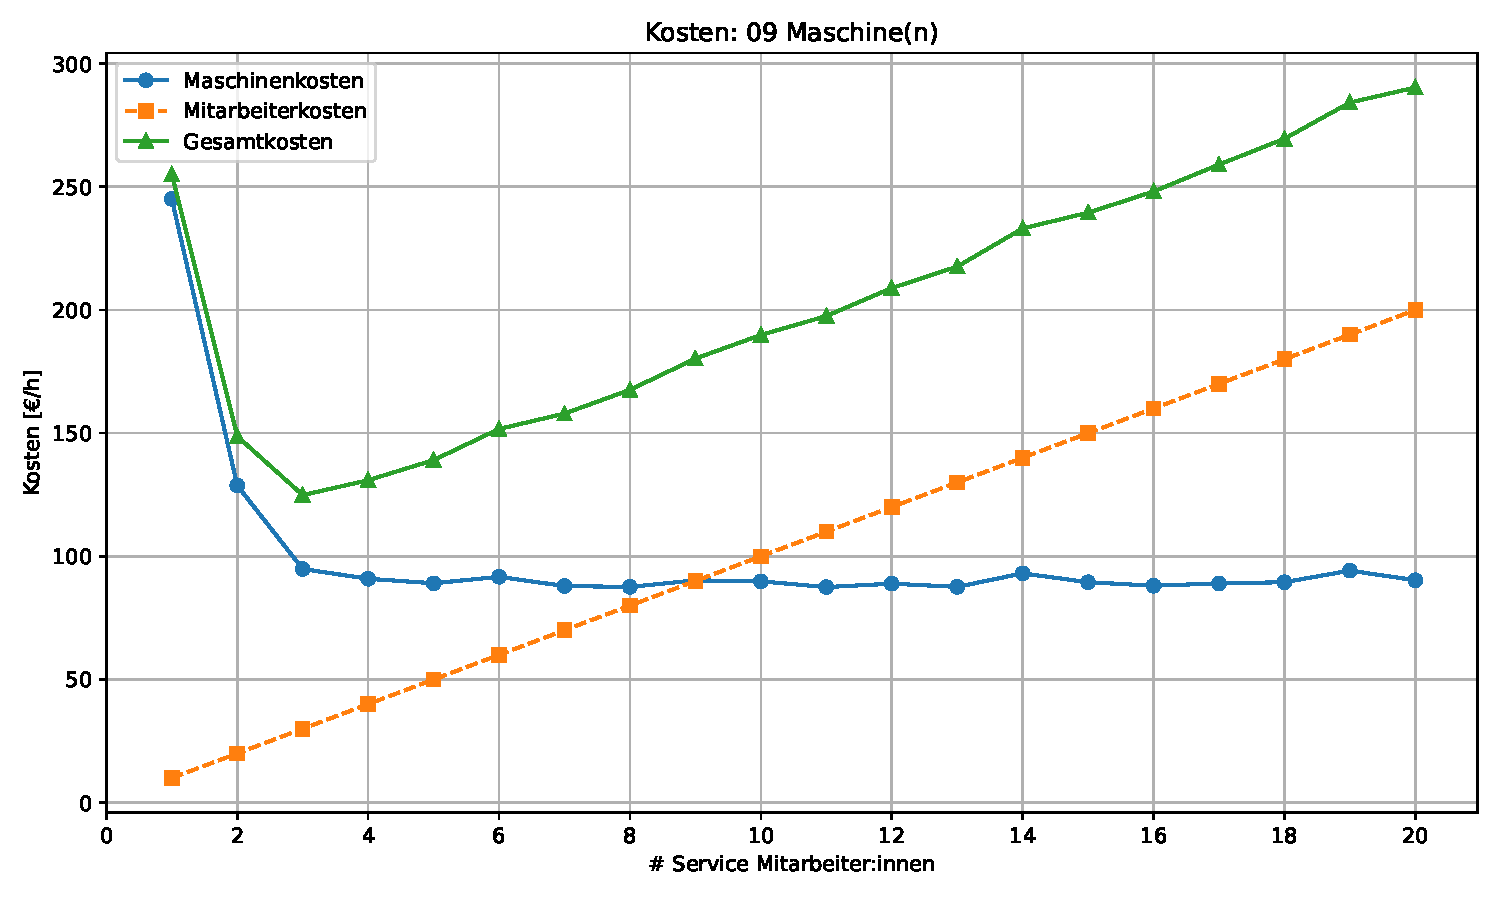
\includegraphics[width=\textwidth]{figures/results/m09_plot}
        \end{figure}
    }
    \only<10>{
        \begin{figure}
            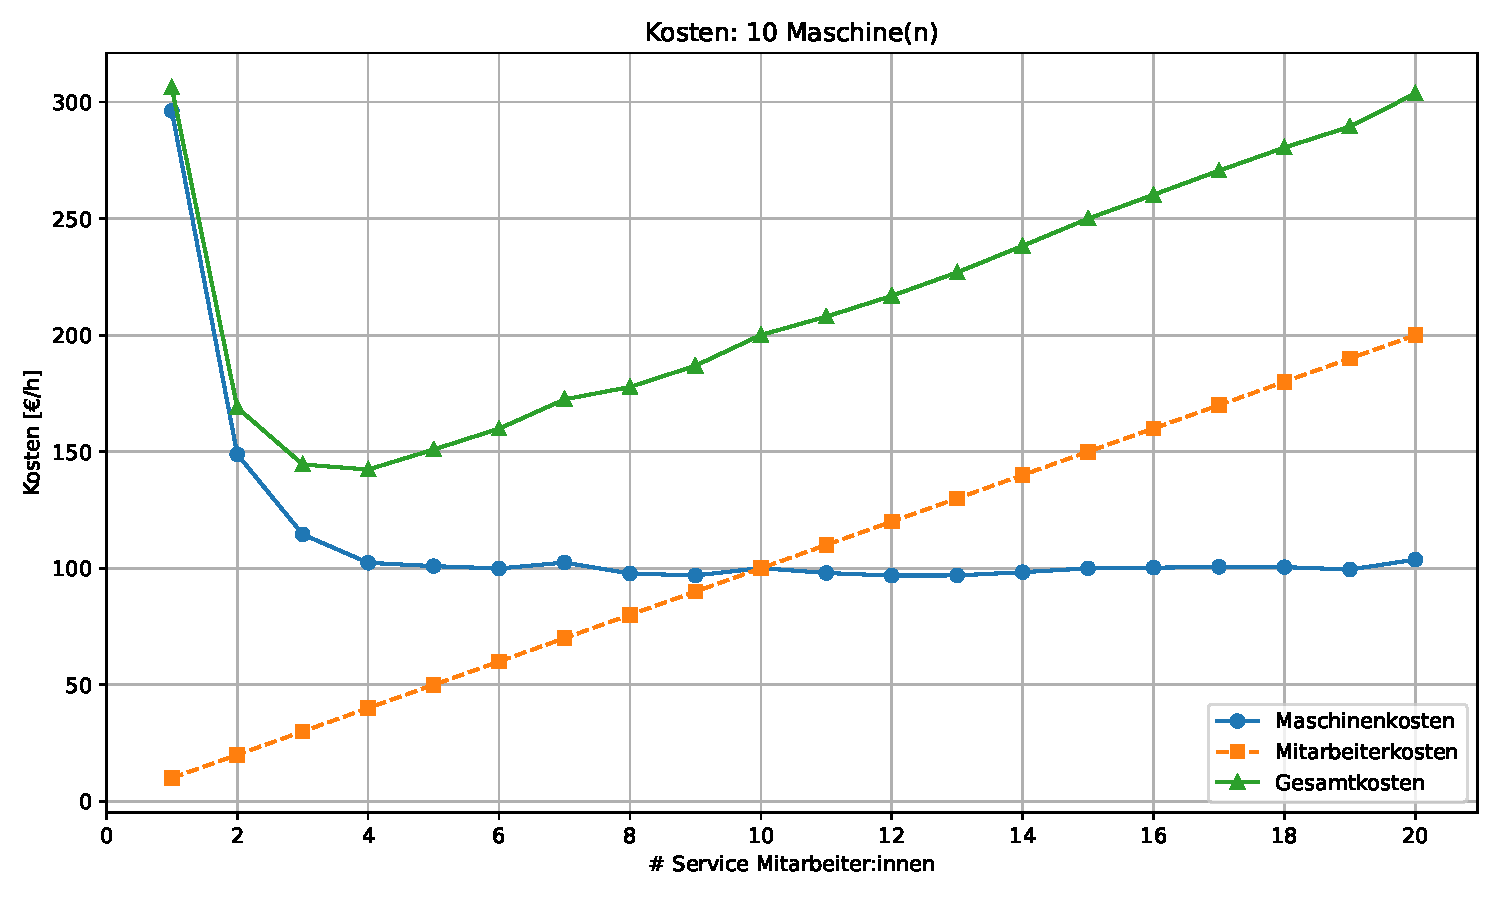
\includegraphics[width=\textwidth]{figures/results/m10_plot}
        \end{figure}
    }
    \only<11>{
        \begin{figure}
            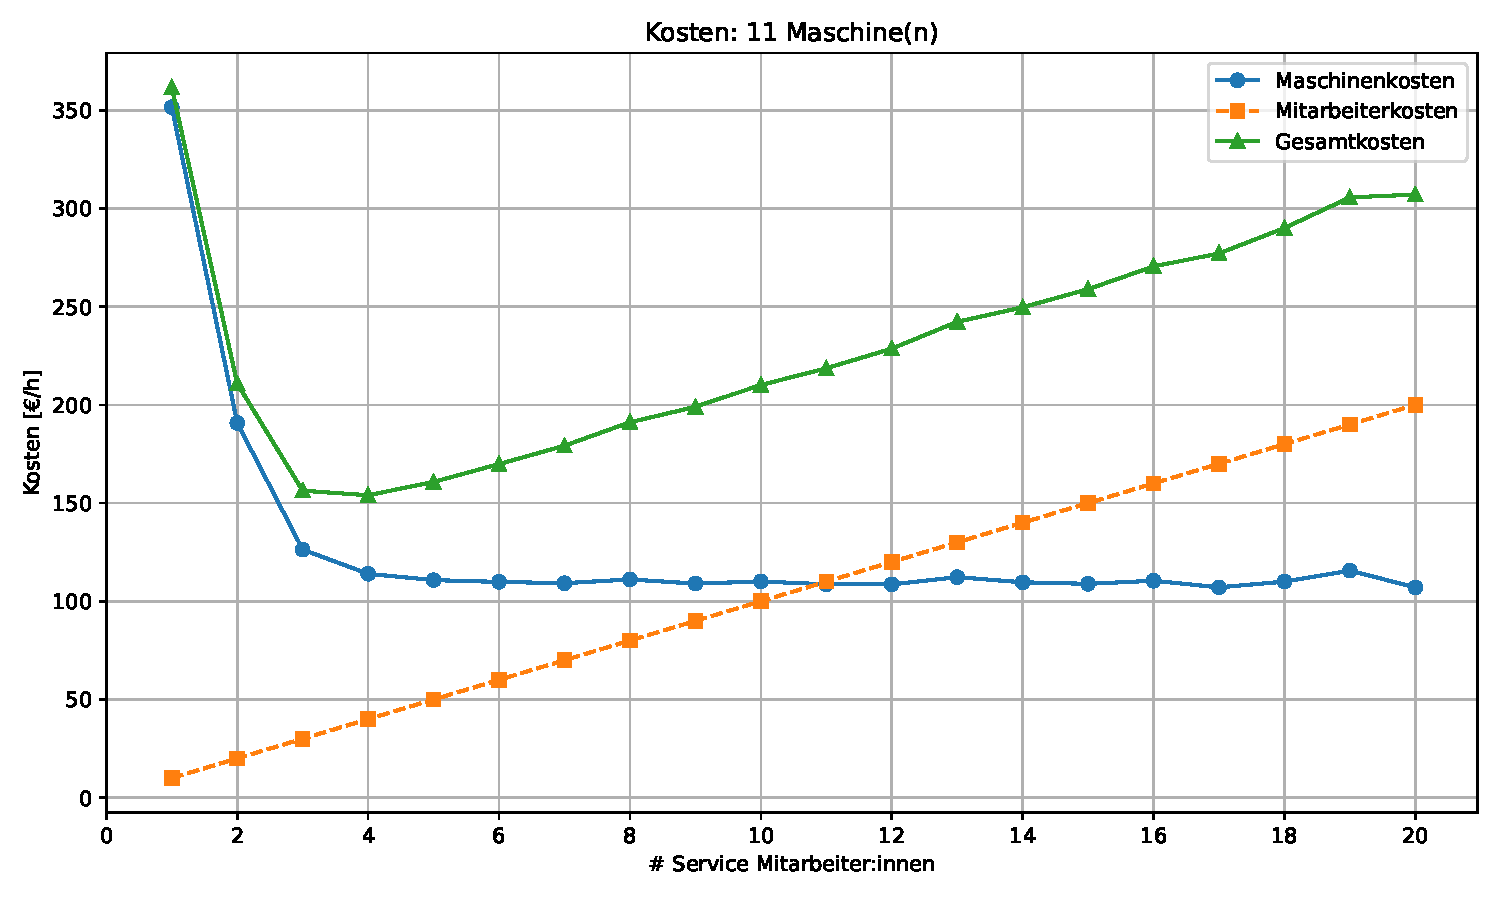
\includegraphics[width=\textwidth]{figures/results/m11_plot}
        \end{figure}
    }
    \only<12>{
        \begin{figure}
            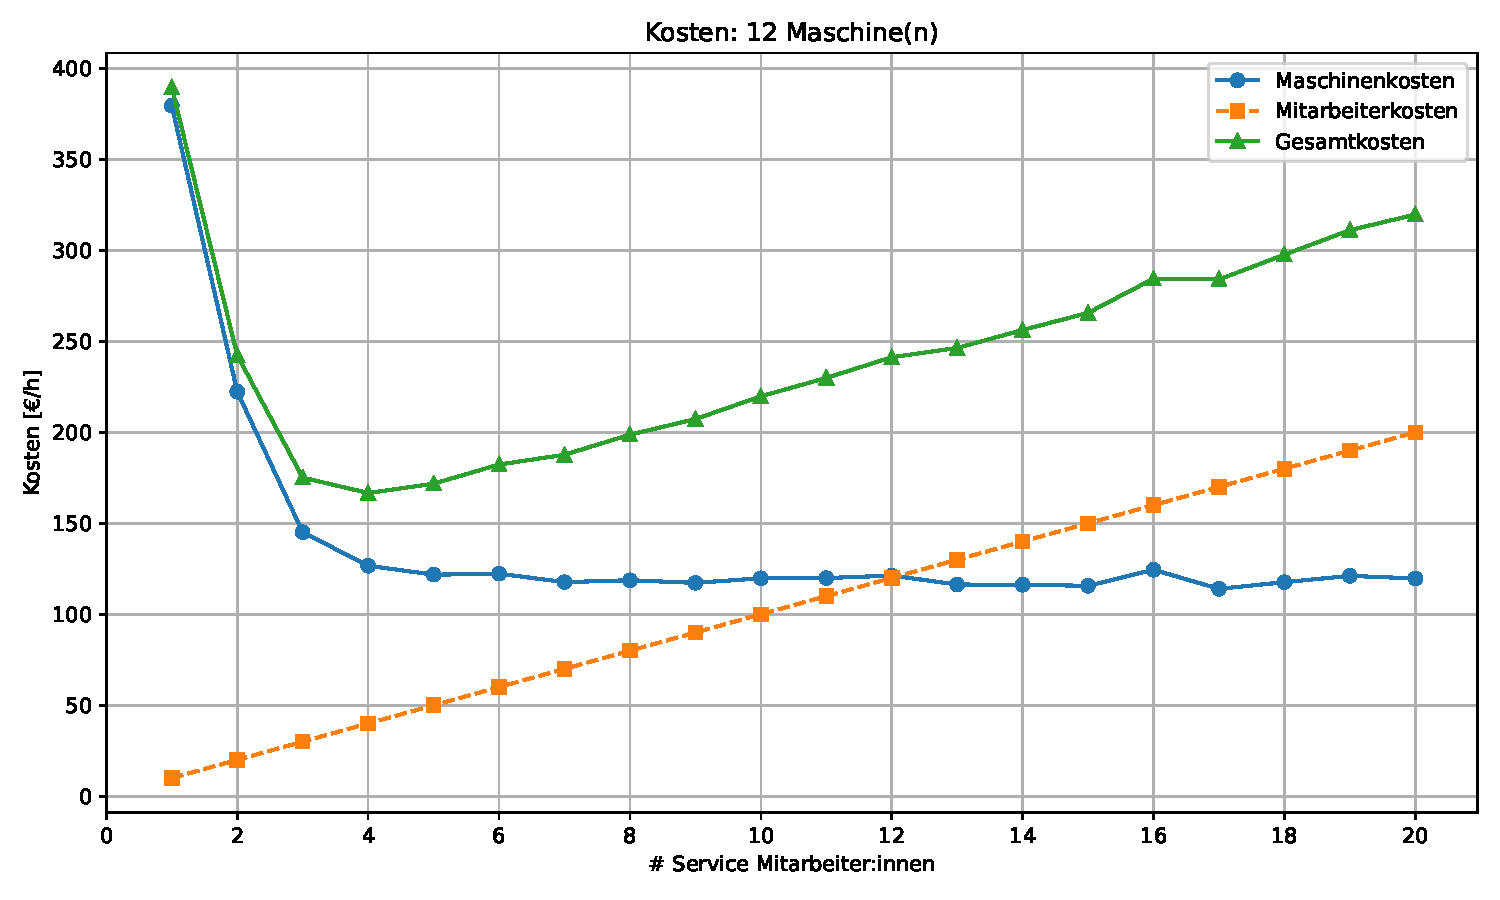
\includegraphics[width=\textwidth]{figures/results/m12_plot}
        \end{figure}
    }
    \only<13>{
        \begin{figure}
            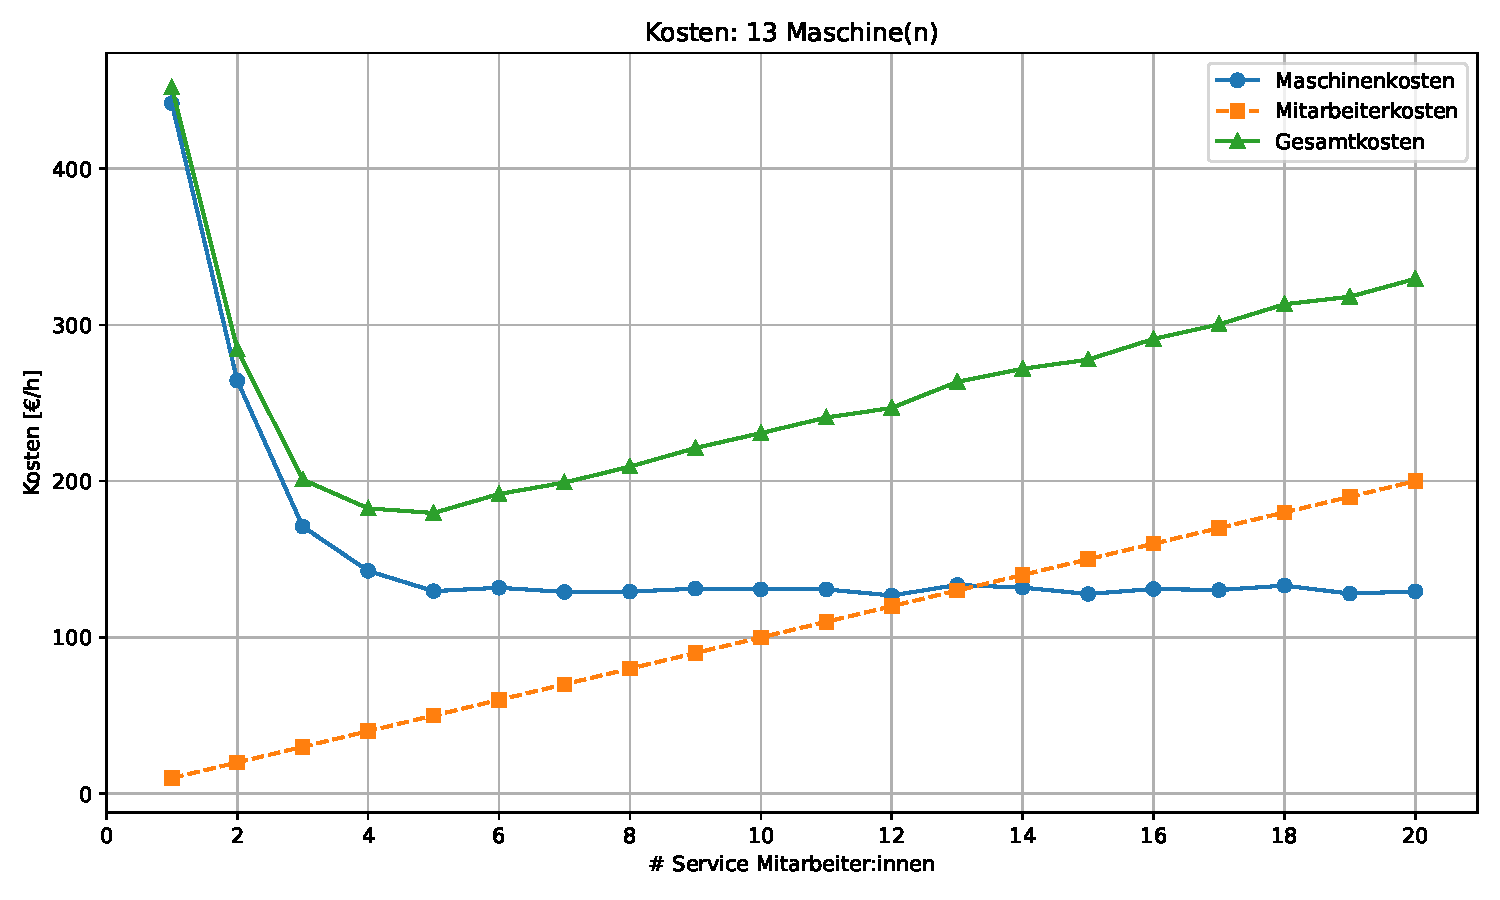
\includegraphics[width=\textwidth]{figures/results/m13_plot}
        \end{figure}
    }
    \only<14>{
        \begin{figure}
            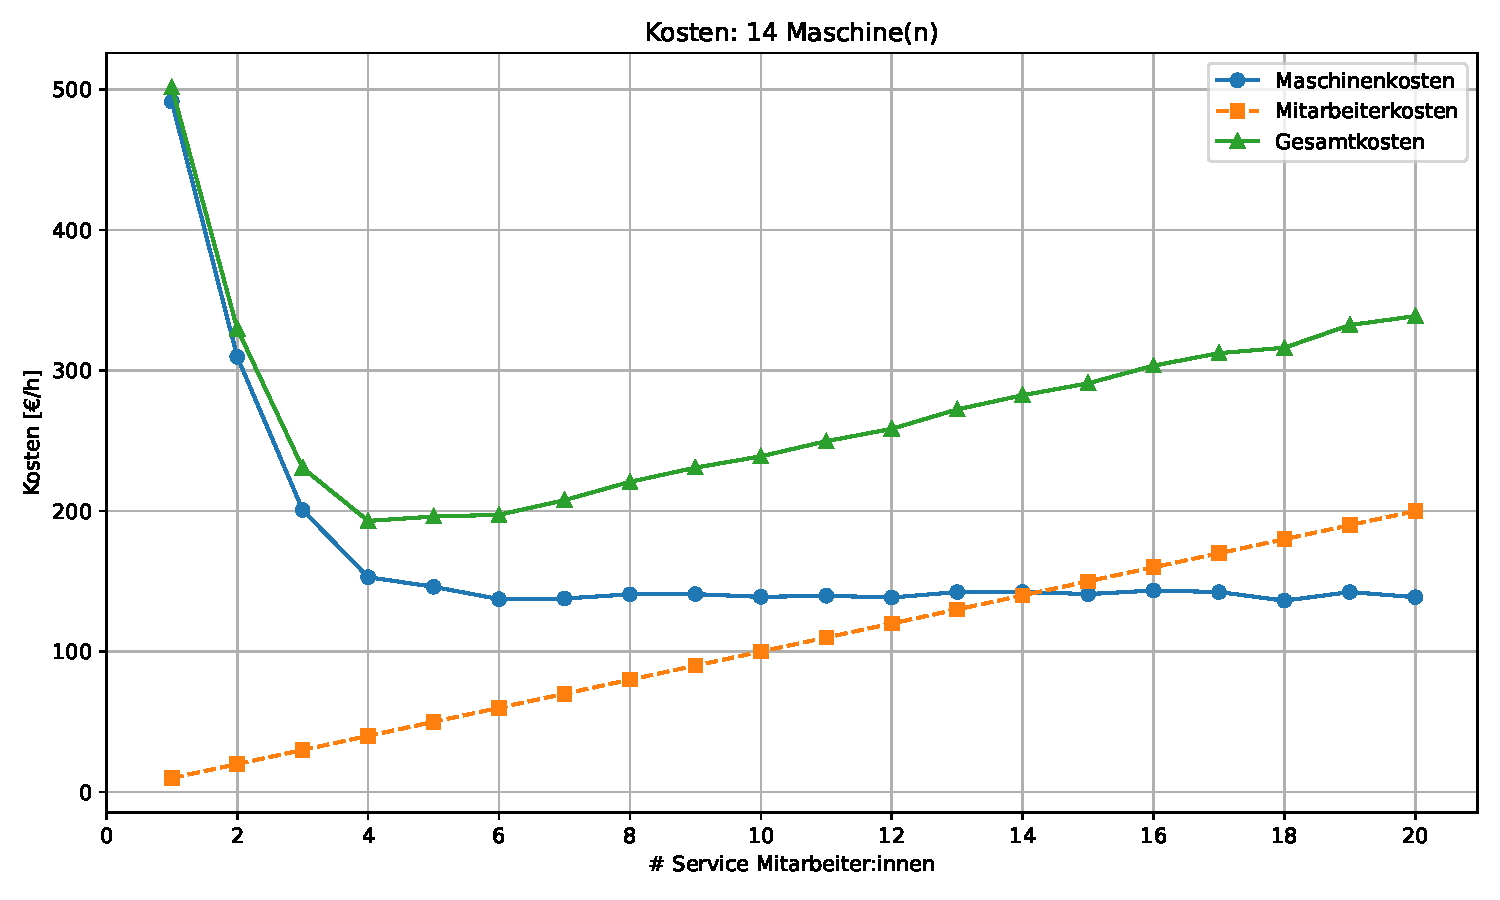
\includegraphics[width=\textwidth]{figures/results/m14_plot}
        \end{figure}
    }
    \only<15>{
        \begin{figure}
            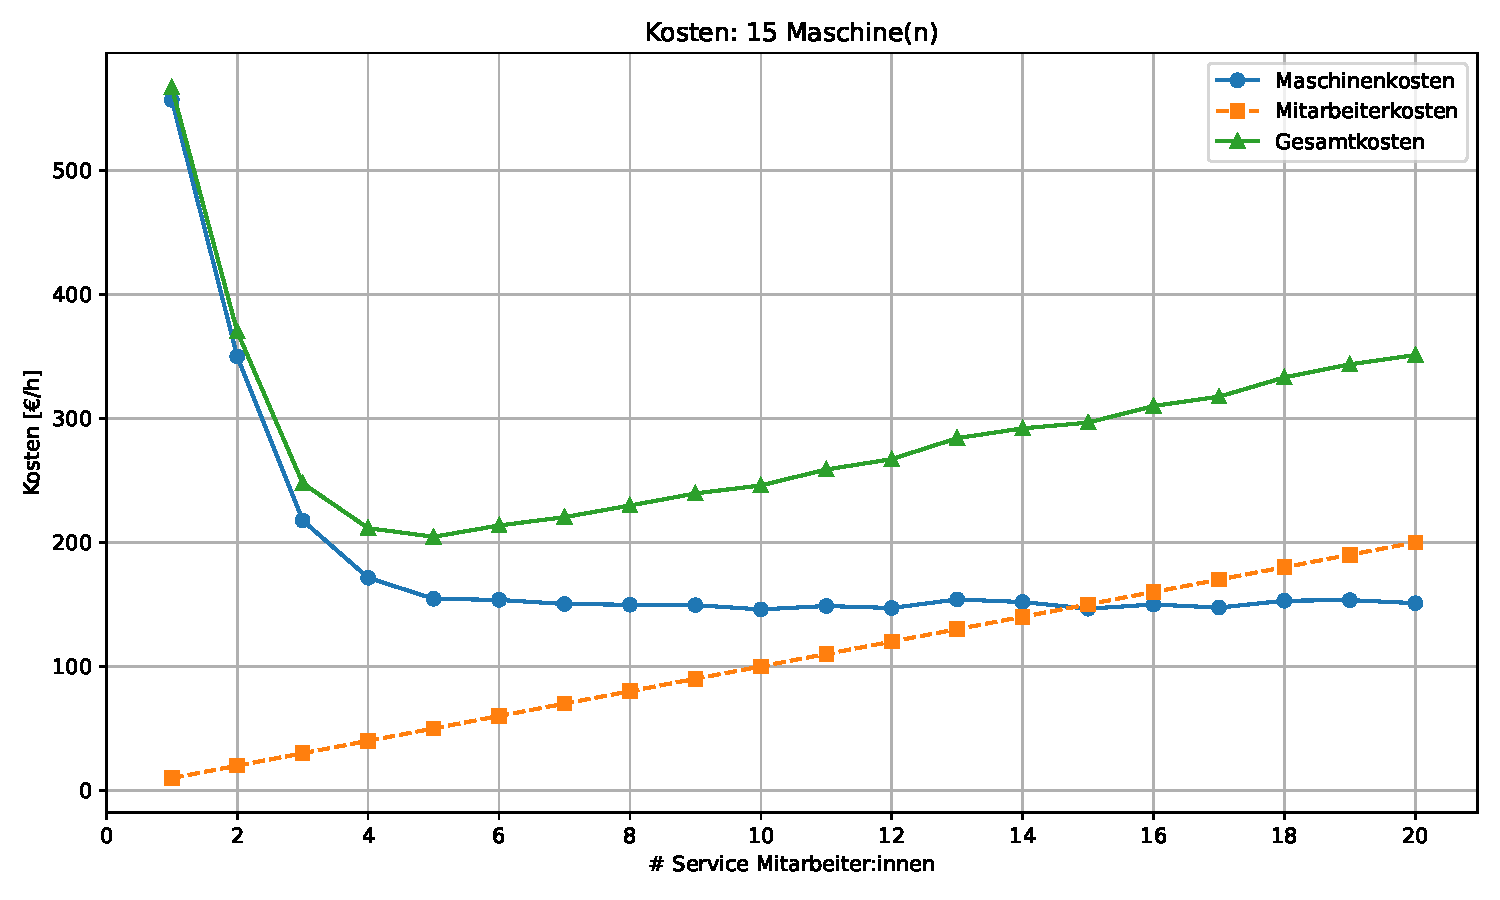
\includegraphics[width=\textwidth]{figures/results/m15_plot}
        \end{figure}
    }
    \only<16>{
        \begin{figure}
            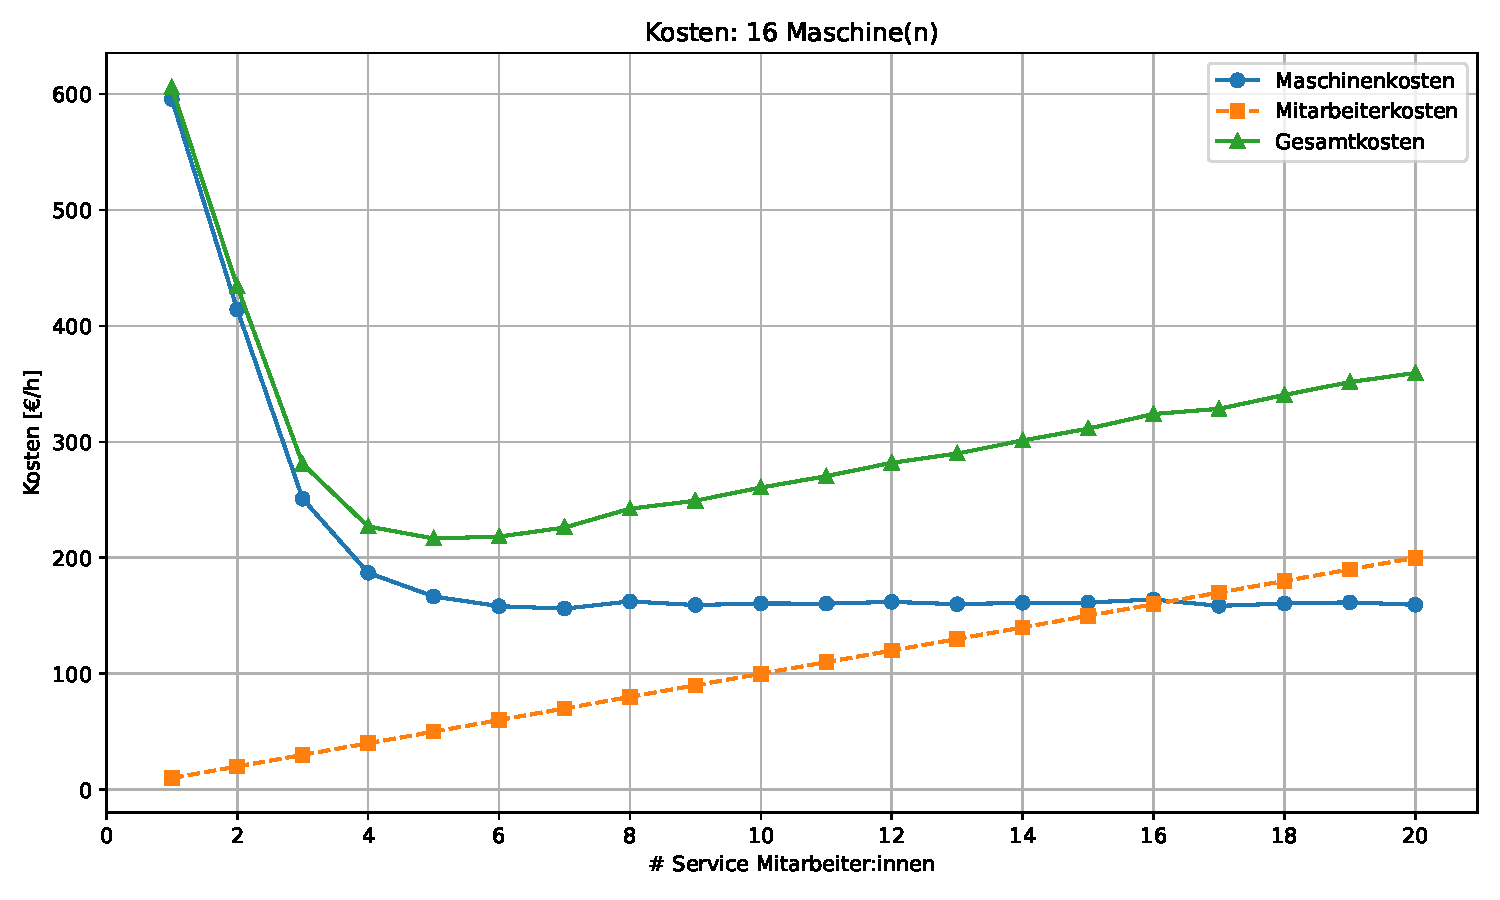
\includegraphics[width=\textwidth]{figures/results/m16_plot}
        \end{figure}
    }
    \only<17>{
        \begin{figure}
            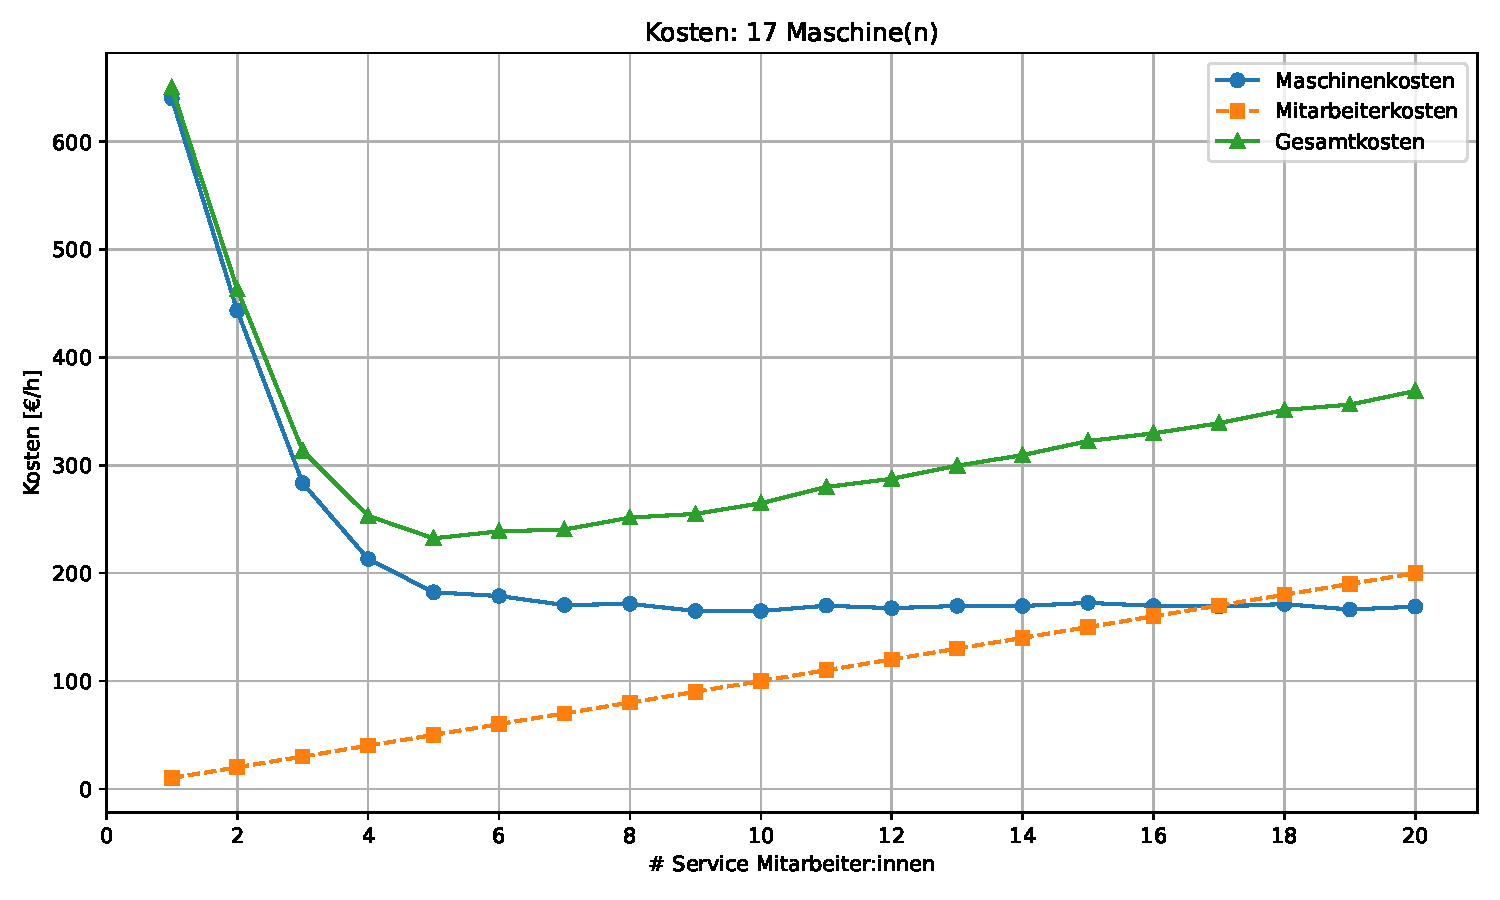
\includegraphics[width=\textwidth]{figures/results/m17_plot}
        \end{figure}
    }
    \only<18>{
        \begin{figure}
            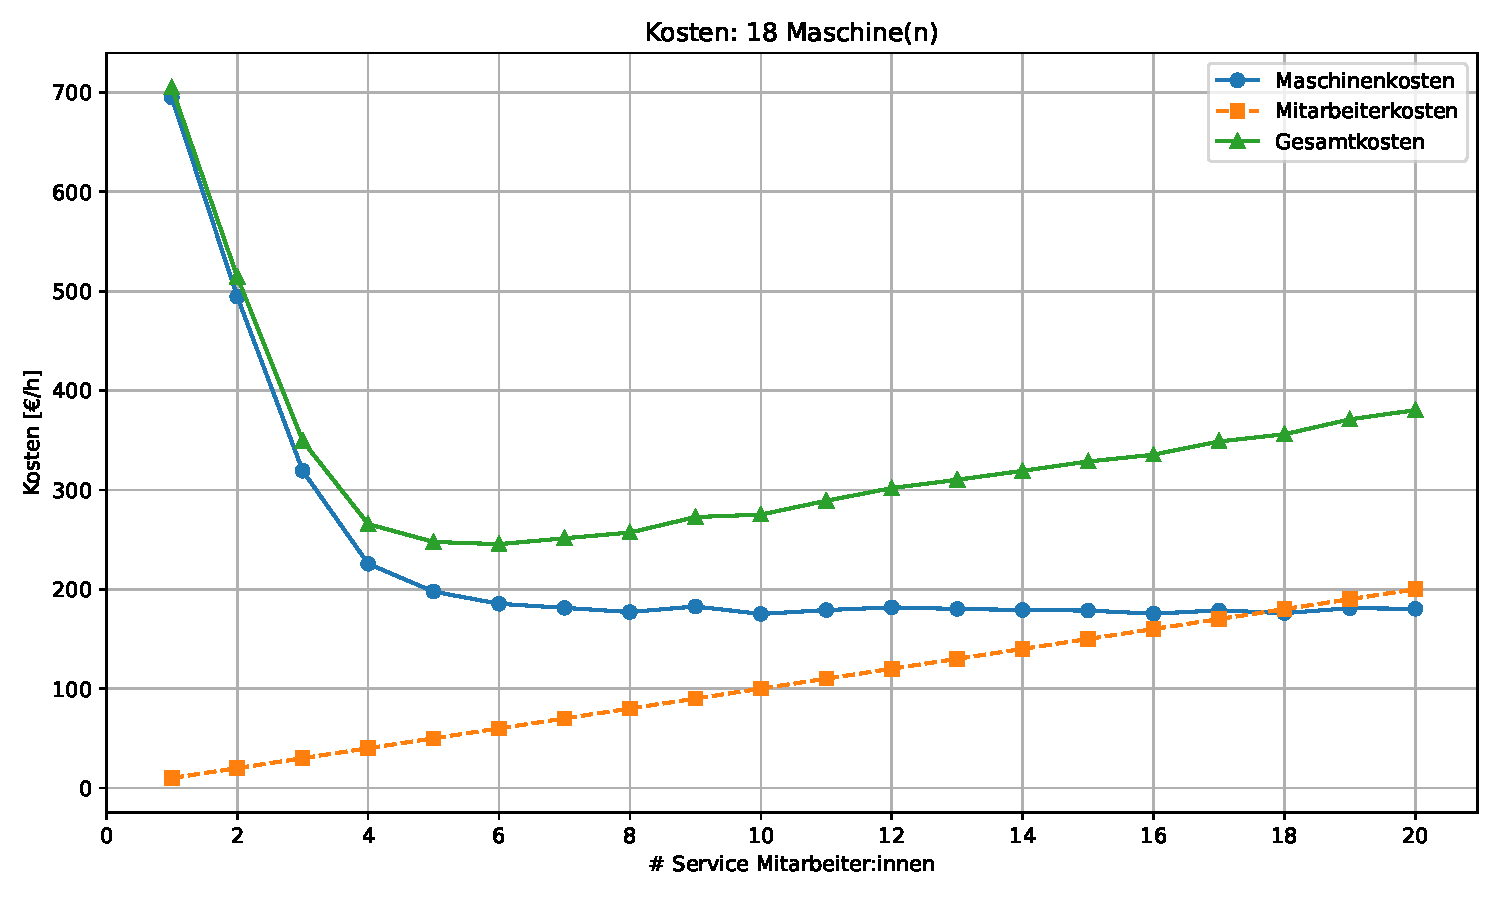
\includegraphics[width=\textwidth]{figures/results/m18_plot}
        \end{figure}
    }
    \only<19>{
        \begin{figure}
            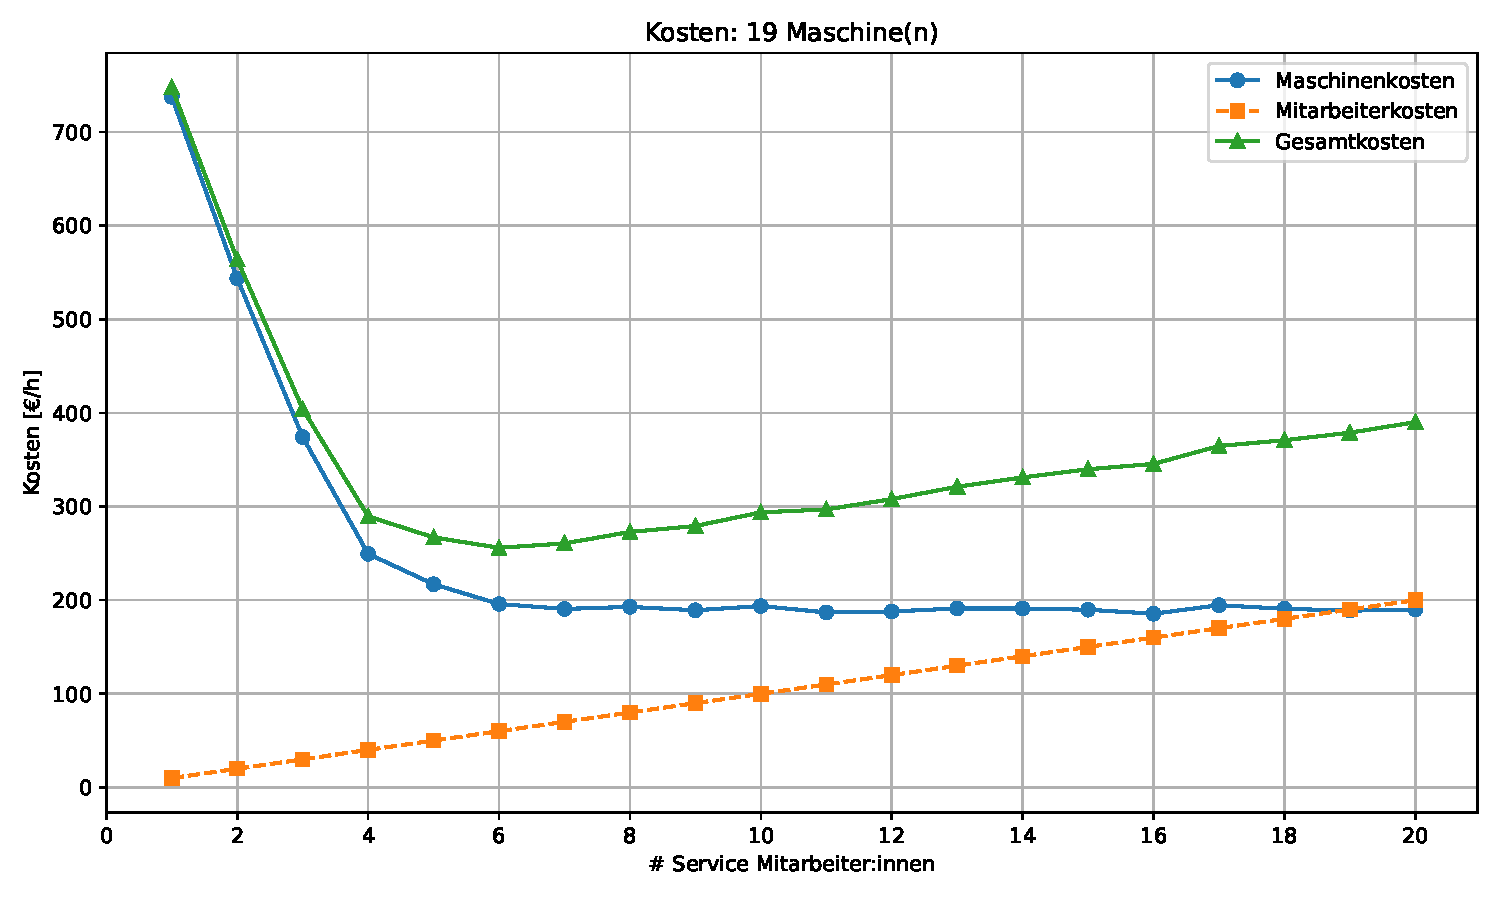
\includegraphics[width=\textwidth]{figures/results/m19_plot}
        \end{figure}
    }
    \only<20>{
        \begin{figure}
            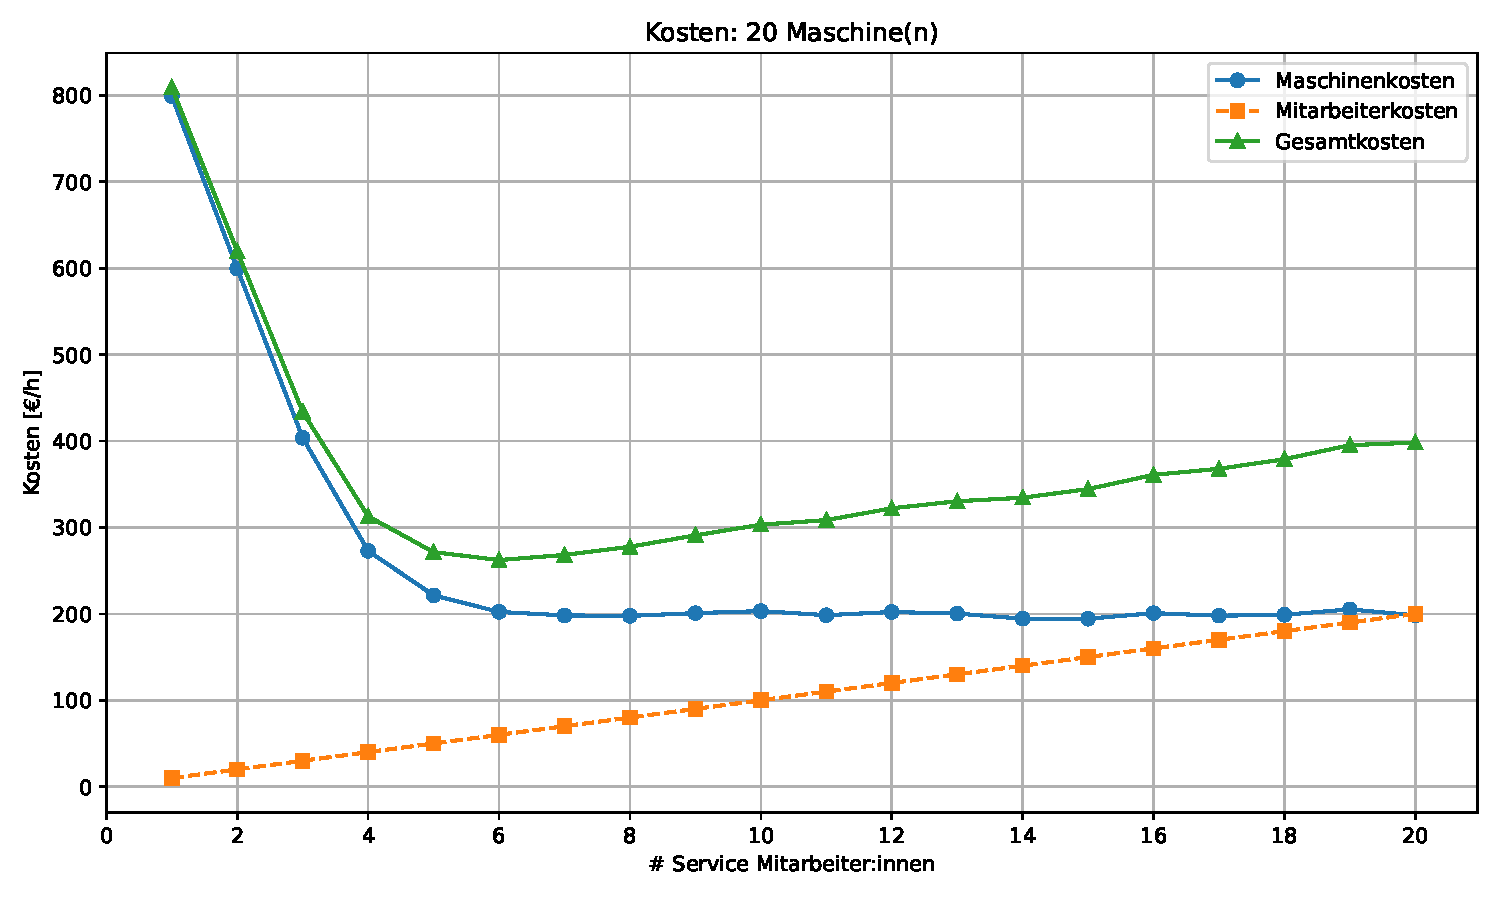
\includegraphics[width=\textwidth]{figures/results/m20_plot}
        \end{figure}
    }
\end{frame}

    \begin{frame}{Interpretation}
        \begin{columns}
            \column{0.48\textwidth}
            Aus den besten Ergebnissen für die jeweilige Anzahl an MitarbeiterInnen
            lässt sich ein Muster erkennen.
            \column{0.48\textwidth}
            \begin{table}
                \begin{tabular}{c|c}
                    Maschinen & MitarbeiterInnen\\\hline
                    1& 1\\
                    2& 1\\
                    3& 2\\
                    4& 2\\
                    5& 2\\
                    6& 2\\
                    7& 3\\
                    8& 3\\
                    9& 3\\
                    10& 4\\
                    11& 4\\
                    $\vdots$ & $\vdots$
                \end{tabular}
            \end{table}
        \end{columns}
    \end{frame}

    \begin{frame}{Regression}
        \begin{figure}
            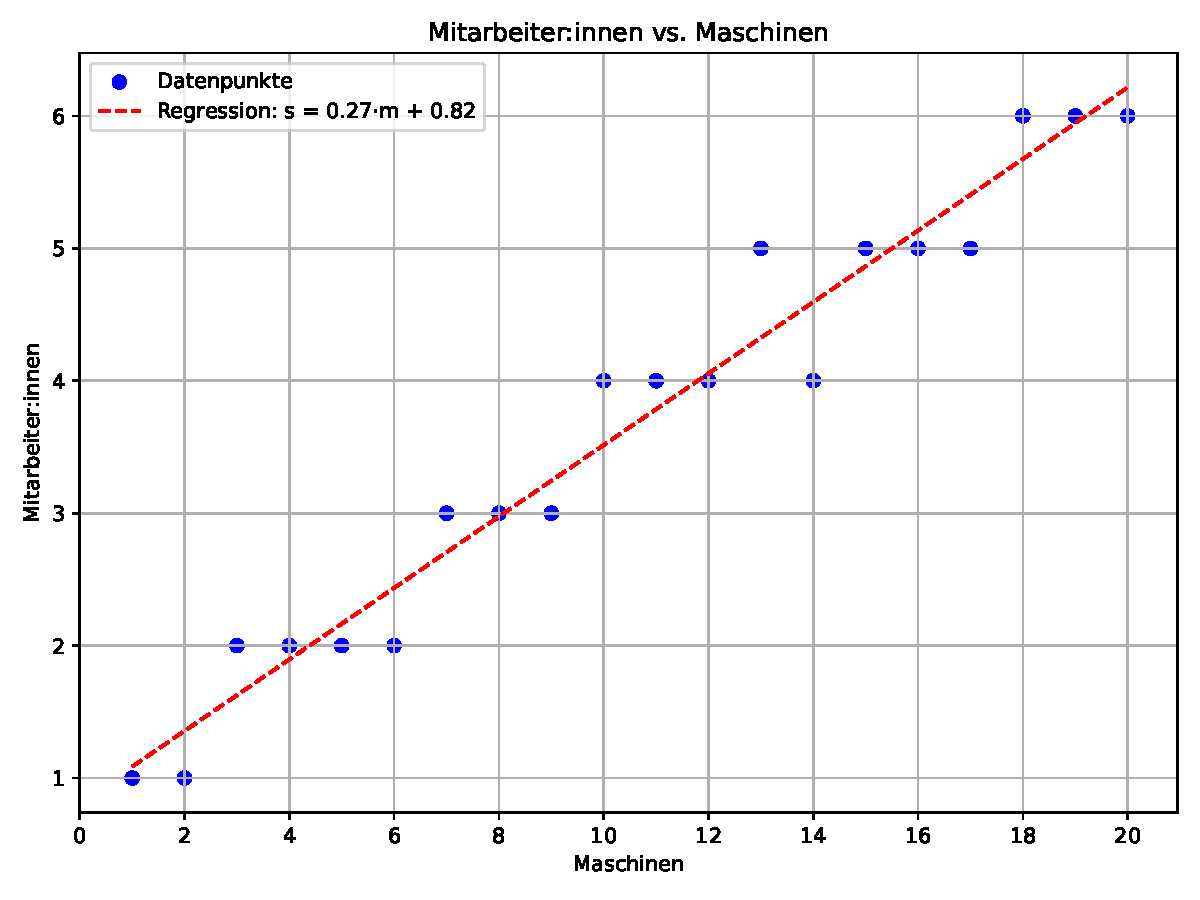
\includegraphics[width=\textwidth]{figures/results/min_costs_all_regression}
        \end{figure}
    \end{frame}

% Section: Conclusion
    \section{Fazit}
    \begin{frame}{Zusammenfassung}
        \begin{itemize}
            \item Entsprechen die Ergebnisse den Erwartungen?\\
            \begin{itemize}
                \item<2-> \textit{Ja}, linearer Anstieg an MitarbeiterInnen war erwartet
            \end{itemize}
            \item Weitere Überlegungen?\\
            \begin{itemize}
                \item<3-> Unterschiedliche Arten von MitarbeiterInnen
                \item<4-> Total Downtime vs. Total Repair Time
                \item<5-> Mehrere Simulation pro Konfiguration (\textit{Problem}: lange Simulationszeit)
            \end{itemize}
        \end{itemize}
    \end{frame}

% Thank you
    \begin{frame}[standout]
        Vielen Dank!\\
        Fragen?
    \end{frame}

\end{document}
